%%
%% Arquivo principal para:
%% - teses de doutorado
%% - dissertações de mestrado
%% - exames de qualificação de mestrado e doutorado
%%
%% NOTA: A PUBLICAÇÃO DESTE MODELO VISA APENAS ORIENTAR OS PÓS-GRADUANDOS
%% NA PREPARAÇÃO DE SEUS TEXTOS. O PPgEE DA UFRN NÃO PROVÊ ASSISTÊNCIA NO
%% USO DAS FERRAMENTAS NECESSÁRIAS AO USO DESTE MODELO (LATEX, XFIG, ETC.)
%%
%% Adelardo Medeiros, dezembro de 2005. Revisado pelos alunos de Metodologia da Pesquisa Científica de 2016.1.

% DEFINIÇÕES GLOBAIS

% Esta primeira linha dá informações gerais sobre o documento.
% PARA A VERSÃO FINAL:
% papel A4, letra grande (12pt), openright (capítulos só iniciam em
% página direita, se necessário incluindo uma página em branco),
% twoside (o documento vai ser impresso em frente e costa)
\documentclass[a4paper,12pt,openright,twoside]{book}
% PARA A QUALIFICAÇÃO E PARA A VERSÃO INICIAL:
% papel A4, letra grande (12pt), openany (capítulos iniciam em
% qualquer página), oneside (o documento vai ser impresso só na frente)
%\documentclass[a4paper,12pt,openany,oneside]{book}

% PACOTES OBRIGATÓRIOS

% Use estes pacotes para poder digitar diretamente as letras com acento
% e para que a hifenização funcione corretamente
\usepackage[utf8]{inputenc}
\usepackage{ae}
% Para usar fontes standard ao invés das do LaTeX (gera melhores PDFs)
\usepackage{pslatex}
% Para a hifenização em português
\usepackage[portuges, brazil]{babel}
% Para que os primeiros parágrafos das seções também sejam indentados
\usepackage{indentfirst}
% Para poder incluir gráficos (figuras)
\usepackage{graphicx}
% Para poder fazer glossário ou lista de símbolos
% Use a segunda opção se quiser incluir na definição do símbolo a
% página e/ou a equação onde ela foi definida
\usepackage[portuguese,noprefix]{nomencl}
%\usepackage[portuguese,noprefix,refeq,refpage]{nomencl}
% Para permitir espaçamento simples, 1 1/2 e duplo
\usepackage{setspace}
% Para usar alguns comandos matemáticos avançados muito úteis
\usepackage{amsmath}
% Para poder usar o ambiente "comment"
\usepackage{verbatim}
% Para poder ter tabelas com colunas de largura auto-ajustável
\usepackage{tabularx}
% Para executar um comando depois do fim da página corrente
\usepackage{afterpage}
% Para formatar URLs (endereços da Web)
\usepackage{url}
% Para reduzir os espaços entre os ítens (itemize, enumerate, etc.)
% Este pacote não faz parte da distribuição padrão do LaTeX.
\usepackage{lib/noitemsep}
% Para as citações bibliográficas
%\usepackage[alf]{abntex2cite}
\usepackage[abbr]{lib/harvard}	% As chamadas são sempre abreviadas
%\harvardparenthesis{square}	% Colchetes nas chamadas
%\harvardyearparenthesis{round}	% Parêntesis nos anos das referências
%\renewcommand{\harvardand}{e}	% Substituir "&" por "e" nas referências

% PACOTES OPCIONAIS

% Para poder incluir arquivos Postscript com cores (do Xfig, por exemplo)
\usepackage{color}
% Para ter células em tabelas que ocupam mais de uma linha
\usepackage{multirow}
% Para poder ter tabelas longas em mais de uma página
%\usepackage{longtable}
% Para poder escrever partes do texto em "n" colunas
%\usepackage{multicol}
% Se você quiser personalizar os cabeçalhos das páginas
%\usepackage{fancyheadings}
% Para incluir algoritmos e listagens de códigos
%\usepackage{listings}
% Para incluir pseudocódigos
\usepackage[portuguese, ruled, linesnumbered]{algorithm2e}
% Capítulos com títulos em um formato "decorado"
\usepackage{lib/capitulos}
% Hiperreferências dentro do texto e montagem dos links do índices dos
% para os leitores de pdf (deve ser o último pacote a ser inserido).
\usepackage[breaklinks]{hyperref}
% Referência correta de ambientes flutuantes (como figuras, tabelas e algoritmos).
\usepackage[all]{hypcap}



% NOVOS COMANDOS

% As definições dos novos comandos estão agrupadas no arquivo "comandos.tex"
% Esta separação é opcional: se você preferir, pode por as definições
% diretamente neste arquivo
% newcommand define novos comandos, que podem passar a ser usados da
% mesma forma que os comandos LaTeX de base.

% Implicação em fórmulas
\newcommand{\implica}{\quad\Rightarrow\quad} %Meio de linha
\newcommand{\implicafim}{\quad\Rightarrow}   %Fim de linha
\newcommand{\tende}{\rightarrow}
\newcommand{\BibTeX}{\textsc{B\hspace{-0.1em}i\hspace{-0.1em}b\hspace{-0.3em}}\TeX}

% Fração com parentesis
\newcommand{\pfrac}[2]{\left(\frac{#1}{#2}\right)}

% Transformada de Laplace e transformada Z
%\newcommand{\lapl}{\makebox[0cm][l]{\hspace{0.1em}\raisebox{0.25ex}{-}}\mathcal{L}}
\newcommand{\lapl}{\pounds}
\newcommand{\transfz}{\mathcal{Z}}

% Não aparecer o número na primeira página dos capítulos
\newcommand{\mychapter}[1]{\chapter{#1}\thispagestyle{empty}}

% Os capítulos sem número
\newcommand{\mychapterast}[1]{\chapter*{#1}\thispagestyle{empty}
\chaptermark{#1}
\afterpage{\markboth{\uppercase{#1}}{\rightmark}}
\markboth{\uppercase{#1}}{}
}

% Seções sem número
\newcommand{\mysectionast}[1]{\section*{#1}
\addcontentsline{toc}{section}{#1}
\markright{\uppercase{#1}}
}

% No tabularx, as celulas devem ser centradas verticalmente
\renewcommand{\tabularxcolumn}[1]{m{#1}}

% Células centralizadas horizontalmente no tabularx
\newcolumntype{C}{>{\centering\arraybackslash}X}

%% Abrevia figuras e tabelas
%\def\figurename{Fig.}
%\def\tablename{Tab.}


%
% As margens
%

% Direção horizontal

% Margem interna
% Nas páginas ímpares
\setlength{\oddsidemargin}{3.5cm}         % Margem real desejada
% Nas páginas pares
\setlength{\evensidemargin}{2.5cm}        % Margem real desejada
% Largura do texto
\setlength{\textwidth}{15cm}
% As margens laterais no LaTeX são sempre 1 polegada maiores do que as
% fixadas. Se foi fixada \setlength{\oddsidemargin}{3.5cm}, a margem
% real seria de 3.5+2.54=6.04cm. Para permitir que você não tenha que
% fazer esta conta, pode usar o número desejado nas linhas anteriores
% e a gente subtrai 1in nas próximas linhas
\addtolength{\oddsidemargin}{-1in}
\addtolength{\evensidemargin}{-1in}
% Note que a margem direita não é fixada diretamente:
% ela é obtida subtraindo-se os outros valores da largura da página.
% 3.5+15+x=21cm (largura A4) -> x = margem externa = 2.5cm

% Direção vertical

% Margem superior (entre o topo da folha e o cabeçalho), altura do
% cabeçalho e distância entre o fim do cabeçalho e o início do texto
\setlength{\topmargin}{2.0cm}             % Margem real desejada
\setlength{\headheight}{1.0cm}
\setlength{\headsep}{1.0cm}
% Altura do texto (sem cabeçalho e rodapé)
\setlength{\textheight}{22.7cm}
% Distância do fim do texto ao rodapé
\setlength{\footskip}{1.0cm}
% A margem superior no LaTeX é sempre 1 polegada maior do que a
% fixada. Se foi fixada \setlength{\topmargin}{2.0cm}, a margem
%real seria de 2.0+2.54=4.54cm. Para permitir que você não tenha que
% fazer esta conta, pode usar o número desejado na linha anterior
% e a gente subtrai 1in na próxima linha
\addtolength{\topmargin}{-1in}
% Note que a margem inferior não é fixada diretamente:
% ela é obtida subtraindo-se os outros valores, sem incluir o
% "footskip", da altura da página.
% 2.0+1.0+1.0+22.7+x=29.7cm (altura A4) -> x = margem inferior = 3cm

%
% O estilo das referências bibliográficas
%

\bibliographystyle{bibliografia/ppgee}

%
% O espaçamento entre linhas
%

% As páginas iniciais são sempre em espaçamento simples
\singlespacing

% Para a criação do glossário (ou lista de símbolos)
\makenomenclature

% Lista de arquivos a serem processados. Estes comandos "includeonly" são
% dispensáveis e devem obrigatoriamente ser comentados na hora de gerar o
% documento definitivo. Eles servem para compilar apenas parte do documento.
% É útil, durante a redação, para que não se tenha de compilar todo o
% documento a cada vez que se faz uma alteração. Por exemplo, se eu estou
% fazendo alterações na dedicatória e as outras partes não têm interesse no
% momento, posso incluir (descomentar) a linha "\includeonly{preambulo}"
%\includeonly{rosto}
%\includeonly{catalograficos}
%\includeonly{preambulo}
%\includeonly{resumos}
%\includeonly{introducao/introducao}
%\includeonly{estilo/estilo}
%\includeonly{matematica/matematica}
%\includeonly{figuras/figuras}
%\includeonly{conclusao/conclusao}
%\includeonly{apendice/apendice}

% Inicia o texto
\begin{document}

% Paginas iniciais (sem numeração)
\pagestyle{empty}

% Página de rosto (capa interna)
%
% ********** Página de Rosto
%

% titlepage gera páginas sem numeração
\begin{titlepage}

\begin{center}

\small

% O comando @{} no ambiente tabular x é para criar um novo delimitador
% entre colunas que não a barra vertical | que é normalmente utilizada.
% O delimitador desejado vai entre as chaves. No exemplo, não há nada,
% de modo que o delimitador é vazio. Este recurso está sendo usado para
% eliminar o espaço que geralmente existe entre as colunas
\begin{tabularx}{\linewidth}{@{}l@{}C@{}r@{}}
% A figura foi colocada dentro de um parbox para que fique verticalmente
% centralizada em relação ao resto da linha
\parbox[c]{3cm}{
\includegraphics[width=\linewidth]{./figuras/UFRN}} &
\begin{center}
\textsf{\textsc{Universidade Federal do Rio Grande do Norte\\
Escola de Ciências e Tecnologia\\
Programa de Pós-Graduação em Ciência, tecnologia e inovação}}
\end{center} &
\parbox[c]{3cm}{
\includegraphics[width=\linewidth]{./figuras/ppgcti-abreveatura}}
\end{tabularx}

% O vfill é um espaço vertical que assume a máxima dimensão possível
% Os vfill's desta página foram utilizados para que o texto ocupe
% toda a folha
\vfill

\LARGE

\textbf{Windbox: Eficiência em gestão operacional de parques eólicos}

\vfill

\Large

\textbf{Danilo Mikael Costa Barros}

\vfill

\normalsize

Orientador: Prof. Dr. Gláucio Bezerra Brandão
% Se não houver co-orientador, comente a próxima linha
% \\[2ex] Co-orientador: Prof. Dr. Beltrano Catandura do Amaral

\vfill

\hfill
\parbox{0.5\linewidth}{\textbf{%
% Descomente as opções que se aplicam ao seu caso
%Proposta de Tema para Qualificação}
Dissertação de Mestrado}
apresentada ao Programa de Pós-Graduação em Ciência, Tecnologia e Inovação da Escola de Ciências, Tecnologia e Inovação - EC\&T da Universidade Federal do Rio Grande do Norte - UFRN,
como parte dos requisitos para obtenção do título de Mestre em Ciências, Tecnologia e Inovação.}
%Doutor em Ciências.}

\vfill

\large

% Este número de ordem deve ser obtido na coordenação do PPgEE
% Corresponde ao número seqüencial da sua tese ou dissertação:
% por exemplo, a 25ª tese de doutorado terá o número de ordem D25
% Evidentemente, este dado não existe para propostas de tema, caso
% em que a próxima linha deve ser comentada.
% Número de ordem PPgCTI: M000

Natal, RN, setembro de 2019

\end{center}

\end{titlepage}


% Ficha catalográfica: os dados catalográficos devem ser fornecidos
% pela BCZM.
% Só são incluídos na versão final da tese ou dissertação. Não são
% incluídos nem na proposta de tema de qualificação nem na versão
% preliminar da tese ou dissertação: nestes casos, comente a próxima linha.
%
% ********** Ficha Catalográfica
%

\newpage

\begin{center}

% Aqui não se usou \vfill porque o \vfill é construído internamente com
% o comando \vspace. Espaços verticais no início da folha com \vspace
% são ignorados. Para que isto não ocorra deve-se usar o \vspace*
% \vspace*{\fill} é como se fosse um \vfill*
\vspace*{\fill}

Divisão de Serviços Técnicos\\[1ex]
Catalogação da publicação na fonte.
UFRN / Biblioteca Central Zila Mamede

\vspace{2ex}

\begin{tabular}{|p{0.9\linewidth}|} \hline
\\
Barros, Danilo Mikael Costa.\\
\hspace{1em} Sobre a Preparação de Propostas de Tema, Dissertações
e Teses no Programa de Pós-Graduação em Engenharia Elétrica e de Computação da UFRN /
Fulano dos Anzóis Pereira - Natal, RN, 2016 \\
\hspace{1em} 23 p. \\
\\
\hspace{1em} Orientador: Gláucio Bezerra Brandão \\
\hspace{1em} Co-orientador: Beltrano Catandura do Amaral \\
\\
\hspace{1em} Dissertação (mestrado) - Universidade Federal do Rio Grande do Norte.
Escola de Ciência, Tecnologia e Inovação. Programa de Pós-Graduação em Ciência, Tecnologia e Inovação. \\
\\
\hspace{1em} 1. Redação técnica - Tese. 2. \LaTeX - Tese.
I. Melo, Sicrano Matosinho de. II. Amaral, Beltrano Catandura do.
III. Título. \\
\\
RN/UF/BCZM \hfill CDU 004.932(043.2) \\ \hline
\end{tabular} 

\end{center}


% Assinaturas da banca, dedicatória e agradecimentos
% Só são incluídos na versão final da tese ou dissertação. Não são
% incluídos nem na proposta de tema de qualificação nem na versão
% preliminar da tese ou dissertação: nestes casos, comente a próxima linha.
%
% ********** Página de assinaturas
%

\begin{titlepage}

\begin{center}

\LARGE

\textbf{Windbox: Eficiência em gestão operacional de parques eólicos}

\vfill

\Large

\textbf{Danilo Mikael Costa Barros}

\end{center}

\vfill

% O \noindent é para eliminar a tabulação inicial que normalmente é
% colocada na primeira frase dos parágrafos
\noindent
% Descomente a opção que se aplica ao seu caso
% Note que propostas de tema de qualificação nunca têm preâmbulo.
Dissertação de Mestrado
%Tese de Doutorado
aprovada em 16 de setembro de 2019 pela banca examinadora composta
pelos seguintes membros:

% Os nomes dos membros da banca examinadora devem ser listados
% na seguinte ordem: orientador, co-orientador (caso haja),
% examinadores externos, examinadores internos. Dentro de uma mesma
% categoria, por ordem alfabética

\begin{center}

\vspace{1.5cm}\rule{0.95\linewidth}{1pt}
\parbox{0.9\linewidth}{%
Prof. Dr. Gláucio Bezerra Brandão (orientador) \dotfill\ PPgCTI/UFRN}

\vspace{1.5cm}\rule{0.95\linewidth}{1pt}
\parbox{0.9\linewidth}{%
Prof. Dr. Jefferson Doolan Fernandes \dotfill\ IFRN}

\vspace{1.5cm}\rule{0.95\linewidth}{1pt}
\parbox{0.9\linewidth}{%
Prof. Dr. Carlos Alexandre Camargo de Abreu \dotfill\ PPgCTI/UFFN}

\end{center}

\end{titlepage}

%
% ********** Agradecimentos
%

% Os agradecimentos não são obrigatórios. Se existem pessoas que lhe
% ajudaram ao longo do seu curso, pode incluir um agradecimento.
% Se não quiser agradecimentos, basta excluir o texto após \chapter*{...}

\chapter*{Agradecimentos}
\thispagestyle{empty}

\begin{trivlist}  \itemsep 2ex

\item À Deus, por ter me dado forças para seguir em frente me levando a essa vitória.

\item Aos meus pai, por toda a ajuda e principalmente por terem me apoiado nas minhas decisões.

\item Ao meu orientador, Professor Gláucio Bezerra Brandão pela paciência, apoio e orientação durante esses anos.

\item Aos demais colegas de pós-graduação, em especial a Elias, George e Ítalo, pelas cômicas conversas sobre empreendedorismo.

\item A todos que fazem e fizeram parte da LogAp Sistemas, pelos conhecimentos trocados e pelo excelente ambiente de trabalho.

\end{trivlist}


%
% O espaçamento entre linhas (ATENÇÃO A ESTA PARTE!)
%
%%%%%%%%%%%%%%%%%%%%%%%%%%%%%%%%%%%%%%%%%%%%%%%%%%%%%%%%%%%%%%%%%%%%%%%%%%%%
% PARA A VERSÃO FINAL:
% Deve ser usado espaçamento simples nas páginas de texto
\singlespacing
% PARA A QUALIFICAÇÃO E PARA A VERSÃO INICIAL:
% Deve ser usado espaçamento 1 1/2 nas páginas de texto
%\doublespacing
%%%%%%%%%%%%%%%%%%%%%%%%%%%%%%%%%%%%%%%%%%%%%%%%%%%%%%%%%%%%%%%%%%%%%%%%%%%%

% Resumo/Abstract
%
% ********** Resumo
%

% Usa-se \chapter*, e não \chapter, porque este "capítulo" não deve
% ser numerado.
% Na maioria das vezes, ao invés dos comandos LaTeX \chapter e \chapter*,
% deve-se usar as nossas versões definidas no arquivo comandos.tex,
% \mychapter e \mychapterast. Isto porque os comandos LaTeX têm um erro
% que faz com que eles sempre coloquem o número da página no rodapé na
% primeira página do capítulo, mesmo que o estilo que estejamos usando
% para numeração seja outro.
\mychapterast{Resumo}

O risco de um investimento em um parque eólico esta fortemente atrelado as diferenças entre a produção efetiva e a produção estimada durante a elaboração do projeto. O acompanhamento do funcionamento dos parques eólicos se faz necessário para que seja garantido o bom desempenho dos mesmo. Neste trabalho será discutido a criação de um produto para uma setor produtivo carente de tecnologia nacional. Será apresentado o Windbox, ferramenta que possibilita o monitoramento contínuo de parques eólicos e que visa o aumento da eficiência desses parques. Além disso será enfatizado a trajetória de criação desta solução assim como os resultados obtidos até o presente momento e as perspectivas futuras.

\vspace{1.5ex}

{\bf Palavras-chave}: Inovação, Processamento de Dados, Energia Eólica,
Coleta de Dados Industriais.

%
% ********** Abstract
%
\mychapterast{Abstract}

The investment risk of a wind farm is heavily bound to the differences between the effective production and the estimated production during the project elaboration.
Monitoring the functioning of wind farms is necessary in order to ensure their good performance. This paper discusses the creation of a product to a productive sector that necesses national technology. It will be presented the Windbox, a tool that allows the continuous monitoring of wind farms and that seeks efficience gain of such wind farms. In addition it will be emphasized the trajectory taken to create this solution as well as the results obtained up to the present moment and future perspectives.

\vspace{1.5ex}

{\bf Keywords}: Innovation, Data Processing, Wind Power,
Industrial Data Collection.


% Paginas introdutórias (com numeração romana)
\frontmatter

% Lista de conteúdo (sumário, gerado automaticamente)
% Aqui, e em todos os itens antes da introdução, o comando \phantomsection é utilizado.
% O seu uso é neecssário para auxiliar o pacote "hyperref" a fazer a referência correta
% dos links do sumário, das listas (de tabelas, figuras, algoritmos) com as páginas 
% respectivas.
% Caso seja tirado, o "hyperref" irá apontar o link do sumário para o abstract, o link
% do sumário para a lista de figuras, o link das listas de figuras para a lista de tabelas,
% e assim sucessivamente.
\phantomsection
\addcontentsline{toc}{chapter}{Sumário}
\tableofcontents

% Lista de figuras (gerada automaticamente)
\cleardoublepage
\phantomsection
\addcontentsline{toc}{chapter}{Lista de Figuras}
\listoffigures

% Lista de tabelas (gerada automaticamente)
\cleardoublepage
\phantomsection
\addcontentsline{toc}{chapter}{Lista de Tabelas}
\listoftables

% Glossário (gerado automaticamente - veja entradas em
% tex/00-introducao/introducao.tex e em tex/02-estilo/estilo.tex)
\cleardoublepage
\phantomsection
\renewcommand{\nomname}{Lista de Símbolos e Abreviaturas}
\markboth{\MakeUppercase{\nomname}}{\MakeUppercase{\nomname}}
\addcontentsline{toc}{chapter}{\nomname}
% O argumento opcional do comando \printnomenclature é a largura deixada
% para os símbolos no glossário. Se seus símbolos são "largos", como
% neste exemplo,  é melhor por mais espaço do que o 1cm que é reservado
% por default
\printnomenclature[1.5cm]

% Páginas do texto principal (com cabeçalho)
\mainmatter
\pagestyle{headings}

% Para facilitar a organização, foi criado um diretório para cada
% capítulo do documento, pois assim os arquivos das figuras ficam
% classificados por capítulos

% Cap. 1 - Introdução
%%
%% Capítulo 1: Modelo de Capítulo
%%

% Está sendo usando o comando \mychapter, que foi definido no arquivo
% comandos.tex. Este comando \mychapter é essencialmente o mesmo que o
% comando \chapter, com a diferença que acrescenta um \thispagestyle{empty}
% após o \chapter. Isto é necessário para corrigir um erro de LaTeX, que
% coloca um número de página no rodapé de todas as páginas iniciais dos
% capítulos, mesmo quando o estilo de numeração escolhido é outro.
\mychapter{Introdução}
\label{Cap:Introducao}

O aproveitamento energético de recursos eólicos no Brasil atravessa um momento de expansão em participação na matriz de energia elétrica nacional, chegando ao final de 2017 a um percentual de participação de 8,1\% segundo a \citeasnoun{boletim-anual-geracao-2017}.

Em outubro de 2017, o Brasil chegou a 12,33 GW de capacidade instalada de energia eólica, com 491 parques eólicos. Ultrapassamos a Itália na capacidade instalada de energia e alcaçamos o 9º lugar no ranking mundial~\cite{abeeolica-boletim-mensal-geracao-out-2017}. A estimativa do governo, que consta no Plano Decenal de Expansão de Energia, é que em 2023 a produção eólica brasileira deverá responder por 11,7\% de toda a produção gerada pelo país. É o tipo de produção de energia que mais cresce no país.

No total acumulado dos anos, o Brasil já tem mais de R\$ 70 bilhões de investimento acumulado e 160 mil empregos em toda a cadeia produtiva. Além de ser uma fonte com baixíssimo impacto de implantação, a eólica não emite CO\textsubscript{2}, o total de emissões evitadas em 2016 foi de 17,81 milhões de toneladas, o equivalente à emissão anual de cerca de 12 milhões de automóveis. Isso vai ajudar o país a cumprir com suas metas de redução da emissão de CO\textsubscript{2} e diversificação da matriz com fontes renováveis complementares.

O Nordeste é referência em produção eólica no Brasil. No dia 23 de junho de 2018 a energia produzida pelos ventos foi responsável por atender 71\% da carga do subsistema do Nordeste, batendo o novo recorde de geração média diária com 7.137 MW médios. Devido a esse bom desempenho, o Nordeste tem sido exportador de energia para o Sudeste/Centro-Oeste \cite{ons-recorde-geracao}.

No ano de 2016 o Rio Grande do Norte foi o estado que apresentou maior geração com 10,59 TWh de energia produzida, representando 33,02\% da geração nacional. Com 125 parques eólicos e 3,4 GW de capacidade instalada de energia eólica, o Rio Grande do Norte é atualmente o primeiro do ranking. O Estado tem cerca de 1.700 aerogeradores. Se considerarmos o que já está contratado para o RN, serão mais 1,2 GW e mais 50 parques até 2020 ~\cite{estados-capacidade-instalada}.

A energia eólico é uma fonte renovável de energia, limpa e inesgotável que sem dúvida, vem crescendo e assumindo uma importante posição no Brasil. Entretanto, para o aproveitamento deste recurso energético são necessários altos níveis de investimentos em parques eólicos. Estes investimento, por sua vez, são rentabilizados de acordo com o desempenho dos aerogeradores que compõem os parques. Procurando minimizar o risco financeiro, os investidores se baseiam em estimativas energéticas do período de produção das usinas, para assim, poder ter uma noção no presente, do seu faturamento futuro. Contudo, ao se comparar a geração prevista com a geração real de um parque, percebe-se que, normalmente, a produção é inferior ao esperado ~\cite{ons2015}. Esses desvios são ocasionados por fatores diversos, em sua maioria relacionados à falhas nos aerogeradores e no sistema elétrico dos parques. Desta forma, é necessário compreender as razões pelas quais existem diferenças entre a geração real obtida e a estimada.

Para impedir os problemas relacionados à falhas, é necessário um planejamento criterioso das manutenções e este tipo de planejamento só é possível mediante o acompanhamento efetivo do desempenho dos parques. Foi pensando nisso que surgiu o Windbox, uma ferramenta na nuvem, no qual os gestores de parques eólicos podem analisar e monitorar o desempenho e a disponibilidade dos seus aerogeradores, assim como, identificar falhas recorrentes e planejar com mais precisão as manutenções. O principal propósito do Windbox é possibilitar o contínuo monitoramento do funcionamento de parques eólicos permitindo detectar desempenhos insatisfatórios, identificar e corrigir as razões destes desvios e, assim, evitar perdas de receita. Além disso, o Windbox possibilita que seja formada uma base de dados e de ensinamentos que podem ser úteis no projeto, construção e operação de outros parques.

Neste trabalho será discutido o desenvolvimento de um projeto de inovação a partir da colaboração de uma empresa privada com uma ICT (Instituição Ciêntifica e tecnológica). Serão demonstrados como o Windbox, um projeto desenvolvido pela LogAp Sistemas em conjunto com o CTGAS-ER (Centro de Tecnologia do Gás e Energias Renováveis), foi criado e introduzido no mercado.

O presente texto está dividido em 6 capítulos. No Capítulo 2 serão apresentados os conceitos básicos que auxiliam o desenvolvimento do trabalho, além de uma visão geral do cenário e da problemática, de maneira a esclarecer as principais características do setor eólico brasileiro e mostrar como o Windbox agrega valor a este mercado.

O capítulo 3 apresentará o desenvolvimento da solução, mostrado todas as suas fases, desde a sua idealização e prototipação até o seu estado atual, apresentando também as dificuldades encontradas e superadas ao longo do caminho.

No Capítulo 4 será dedicado a gestão da inovação, no qual será discutida a atuação do CInO (\textit{Chief Innovation Officer}) e a sua importância para o desenvolvimento do projeto apresentado.

Por fim, o Capítulo 5, serão apresentados os resultados do projeto, considerações finais e a perspectivas para o futuras.


%\section{Organização do texto}
%
%O fecho do capítulo introdutório muitas vezes apresenta uma ideia
%global do trabalho, mostrando o que vai ser tratado nos capítulos
%subsequentes.





% Cap. 2 - Fundamentação Cientifico-tecnológica
%%
%% Capítulo 2: Regras gerais de estilo
%%

\mychapter{Fundamentação científico-tecnológica}
\label{Cap:fundamentacao}

\section{Contextualização e problema}
\label{contextualização}


% Falar um pouco sobre o cenário mundial de eólica

% Falar sobre o problema com desempenho das máquinas

% Falar das tecnologias utilizadas

% Falar da robustez do sistema

% Falar do valor agregado


O Brasil recebe destaque no cenário mundial pelo elevado potencial eólico e pelo volume de geração de energia por fonte eólica, que tem crescido consideravelmente nos últimos anos. Com 508 usinas no total, o ano de 2017 terminou com 12,77 GW de potência eólica instalada, o que representou um crescimento de 18,87\% de potência em relação a dezembro de 2016, quando a capacidade instalada era de 10,74 GW \cite{boletim-anual-geracao-2017}.

Em 2017 foram instalados 6,84 GW de potência, considerando todas as fontes de geração de energia elétrica. Desse crescimento, 47,86\% corresponde a fonte hidroelétrica e 29,62\% a fonte eólica. Com esse acréscimo de 2,03 GW de capacidade instalada, o total eólico permitiu para a fonte uma participação de 8,10\% da matriz elétrica brasileira, como pode ser observado no gráfico \ref{Fig:matriz-energetica-brasileira}, que apresenta a participação de todas as fontes de geração na matriz elétrica brasileira no final de 2017 \cite{boletim-anual-geracao-2017}.

\begin{figure}[htbp!] \begin{center}
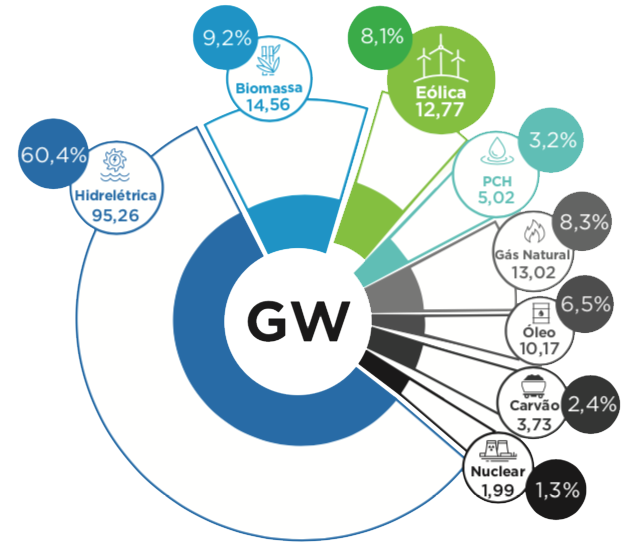
\includegraphics[width=0.75\linewidth]{./figuras/matriz-energetica-brasileira}
\caption{Matriz energética brasileira}
\label{Fig:matriz-energetica-brasileira}
\end{center} 
\end{figure}

Sendo um dos países que mais investe em energia eólica no mundo, o Brasil também é considerado um dos mais atrativos para investimentos em energias renováveis. A fonte eólica, sozinha, foi responsável por cerca de 80\% dos investimentos em renováveis no país de 2005 até 2015 \cite{CENARIO}. Um dos maiores motivos do alto investimento em energia eólica no Brasil é o alto valor do fator de capacidade proporcionado pelos ventos brasileiros. O fator de capacidade aponta o aproveitamento do vento para produção de energia e é representado pela proporção entre a geração efetiva da usina em um intervalo de tempo e a sua potência instalada. Em 2017 o valor médio do fator de capacidade no Brasil foi de 42,9\%, tendo atingido maior fator mensal médio em setembro, com 60,6\%, enquanto que no restante do mundo a média do é de 24,7\%.



O desempenho dos empreendimentos eólicos é fator determinante na definição do ritmo de crescimento e participação da fonte eólica na matriz elétrica brasileira e, consequentemente, no alcance das metas fixados pelo Governo.

O contributo social desta pesquisa é fornecer uma ferramenta que irá possibilitar o aumento da eficiência dos parques, conferindo, consequentemente, maior competitividade para a fonte eólica frente às demais fontes de geração, o que pode estimular a modicidade tarifária, a qual preconiza o consumo de energia mais barata para o cidadão brasileiro. Além disso, incentivar a expansão de fontes renováveis de energia, que não agridem o meio ambiente, é contribuir para o bem-estar humano.






Não há um número mínimo ou máximo de páginas para propostas de tema,
dissertações ou teses. Entretanto, se o seu documento for muito menor
do que a média pode transmitir uma ideia de falta de conteúdo a
apresentar. Por outro lado, um documento muito grande corre o risco de
só conseguir a atenção total do leitor no seu início, fazendo com que
as partes mais importantes, que geralmente estão no final do
documento, não sejam devidamente consideradas. Apenas para servir como
parâmetro, estão indicados a seguir os limites usuais quanto ao número
de páginas\footnote{Uma folha corresponde a uma página em impressão em
face simples e a duas páginas em impressão em face dupla} dos
documentos do PPgEEC da UFRN, adotando as margens e os espaçamentos
definidos neste modelo:
\begin{itemize}
\item Proposta de tema para exame de qualificação de mestrado:
entre 20 e 40 páginas
\item Proposta de tema para exame de qualificação de doutorado:
entre 30 e 50 páginas
\item Dissertação de mestrado:
entre 50 e 100 páginas
\item Tese de doutorado:
entre 80 e 150 páginas
\end{itemize}

O tamanho padrão para a fonte é de 12pt.  Para facilitar a escrita de
comentários, sugestões e correções da banca, recomenda-se o espaçamento
1.5 entre as linhas do texto e a impressão em um único lado da folhas
para os seguintes documentos:
\begin{itemize}
\item Proposta de tema para exame de qualificação;
\item Versão inicial de dissertação de mestrado; e
\item Versão inicial de tese de doutorado.
\end{itemize}
Para as versões finais de teses e dissertações, onde se busca uma
melhor qualidade visual e tipográfica do texto, deve-se utilizar
espaçamento simples entre as linhas e a impressão nos dois lados da
página.

As margens devem seguir os valores adotados neste documento, que podem
ser verificados no arquivo \texttt{principal.tex}. É importante notar
que, na versão final de teses ou dissertações, recomenda-se a
impressão nos dois lados da página. Por esta razão, a margem direita
em páginas pares deve ter o mesmo valor que a margem esquerda em
páginas impares e vice-versa, para que a encadernação fique
correta. Também em razão da impressão em frente e verso, os capítulos
devem sempre começar em uma página de número ímpar, com a eventual
inclusão de uma página em branco. O \LaTeX\ se encarrega de fazer
automaticamente estes ajustes.

\section{Robustez do sistema}
\label{RobustezSistema}

Documentos do porte de uma tese ou dissertação devem ser subdivididos
em capítulos. O capítulo deve conter uma introdução e um fecho.

A introdução do capítulo fornece ao leitor uma breve descrição do que
será tratado no capítulo e não forma uma seção: para exemplificar, a
introdução deste capítulo é o parágrafo que precede a primeira seção.

O fecho do capítulo apresenta comentários finais sobre o que foi
desenvolvido no capítulo e/ou faz uma ligação com o que será visto no
capítulo seguinte; normalmente é colo cado em uma seção específica,
denominada ``Comentários Finais'', ``Conclusões'', ``Resultados'',
``Avaliação Final'' ou qualquer outra denominação que se adéque ao
texto.

Capítulos são divididos em seções. O número ideal de seções é
impossível de se precisar. Entretanto, um capítulo com uma única seção
provavelmente deve ser agregado ao capítulo anterior ou posterior. Um
capítulo com quinze seções provavelmente deve ser subdividido em dois
capítulos.

Capítulos, seções e subseções devem ser rotulados para que possam ser
referenciados em qualquer parte do texto.  Isto é feito com o comando
\verb|\label{}|, que deve ser colocado logo após (nunca antes) o
comando que criou a seção, capítulo, etc. O parâmetro do comando
\texttt{label} é o nome simbólico que será usado para se fazer
referência a esta entidade dentro do texto, com o comando
\verb|\ref{}|. O nome pode ser qualquer coisa, mas não pode conter
acentos, por exemplo. Neste documento nós utilizamos a convenção de
prefixar os rótulos dos capítulos com \texttt{Cap:}, das seções com
\texttt{Sec:}, das equações com \texttt{Eq:} e assim por diante, mas
esta convenção não é obrigatória. Veja a seguir um exemplo de
utilização das referências cruzadas:
% quotation é um ambiente para citações, que ficam "recuadas" em
% relação ao resto do texto
\begin{quotation}
\dots no capítulo~\ref{Cap:Introducao} apresentamos um modelo de
capítulo de tese.
\end{quotation}
Note que, no código fonte deste trecho de frase, o espaço entre a palavra
\texttt{capítulo} e o comando \verb|\ref{}| foi escrito com
um \texttt{\~{}} e não com um espaço normal. O \texttt{\~{}} é o
comando \LaTeX\ para criar um espaço onde não se pode mudar de linha,
pois ficaria estranho se o texto ``no capítulo'' estivesse no fim de
uma linha e o número \ref{Cap:Introducao} no início da outra linha.

Existe uma particularidade no código fonte do parágrafo anterior. Para
se escrever:
\begin{quotation}
\dots o comando \LaTeX\ para criar\dots
\end{quotation}
se colocou depois do comando \verb|\LaTeX| um espaço
precedido de uma contrabarra, ao invés de um espaço normal. Isto porque
espaços depois de comandos são ignorados pelo \LaTeX; com um espaço
% Na linha anterior não houve necessidade do espaço com contrabarra
% depois do comando \LaTeX, pois ele é seguido por um ; e não um espaço
normal as palavras ficariam ligadas:
\begin{quotation}
\dots o comando \LaTeX para criar\dots
\end{quotation}
Ao invés do espaço precedido pela contrabarra, poder-se-ia também
utilizar um \texttt{\~{}}. A diferença é que neste caso o \LaTeX\ não
poderia fazer uma quebra de linha entre as palavras.


% Cap. 3 - Desenvolvimento da solução
%%
%% Capítulo 2: Expressões matemáticas
%%

\mychapter{Trabalhos relacionados}
\label{Cap:TrabalhosRelacionados}

Visando esse cenário de expansão de geração de energia eólica no Brasil, e a posição estratégica da região Nordeste, em específico o estado do Rio Grande Norte, a LogAp Sitemas une a sua  expertise no desenvolvimento de software de análises de dados industriais, com a expertise técnica do CTGAS-ER em energias renováveis, especificamente em energia eólica, para desenvolverem juntos o Windbox. Além das dificuldades dos gestores e operadores em realizarem análises de disponibilidade e desempenho  e detecção prévia de falhas dos ativos físicos dos parques eólicos, julgamos unir os principais elementos necessários para construção de uma solução que irá contribuir para uma maior eficiência dos parques eólicos.



Atualmente o sistema Athenas Eólico possui os seguintes módulos implementados:
\begin{itemize}
	\item Análise de curva de potência: este módulo permite comparar a curva de potência contratual do aerogerador com a curva real com base em especificação da norma IEC 61400-12-1, possibilitando ao gestor maior respaldo nas negociações das manutenções efetuadas pelo fabricante durante o período de garantia do parque.
	\item Análise de Eventos/Alarmes: este módulo possibilita uma análise de disponibilidades dos aerogeradores do parque de modo a identificar os principais eventos que contribuem para paradas não programadas.
	\item Análise de produção energética considerando a curva certificada da unidade aerogeradora e do parque eólico de acordo com a norma IEC 61400-26-2: módulo possibilita uma análise da produção de energia do parque, detalhando informações de produção potencial, real e estimativa de perda em conjunto com indicadores de disponibilidade e desempenho do parque.
\end{itemize}
Assim, o presente projeto visa o amadurecimento do sistema integrado Athenas Eólico, tanto do ponto de vista técnico e científico, como do ponto de vista mercadológico. De modo a agregar desenvolvimentos de novas funcionalidades como: notificação de eventos de alerta, gerenciamento de manutenções, diagnósticos preditivo de falhas, construção de base de conhecimento e demais módulos descritos nos objetivos específicos.

Espera-se ao final do projeto que a solução de sistema integrado seja capaz de oferecer aos gestores, operadores e investidores de empreendimentos eólicos os seguintes benefícios:

\begin{enumerate}
\item Apoio na decisão, planejamento e gestão da Operação e Manutenção (O\&M) do parque eólico.
\item Fiscalização e monitoramento do desempenho e disponibilidade do parque eólico em comparação com o contratado com o fabricante em termos de curvas de certificação.
\item Otimização da produção com aumento da disponibilidade e performance, maximizando a produção.
\item Análise anemométrica nas fases de campanhas de medição anemométrica e de operação do parque.
\item Controle de manutenções corretivas e base de conhecimento para respaldo de melhor solução para determinada problemática.
\item Análise de dados independente do fabricante.
\item Relatórios automatizados de prestação de conta para investidores e diretores.
\item Relatórios automatizados para órgãos regulatórios como EPE e ONS.
\item Mitigação de riscos regulatórios (Multas).
\end{enumerate}




Nos trabalhos relacionados, coloque a essência dos trabalhos no domínio abordado (com referências bibliográficas). Isto não inclui citações específicas e particulares para trabalhos anteriores (seus e de outros), mas sim, algo mais genérico, por categoria ou características (por exemplo, classificar os trabalhos segundo as técnicas empregadas). É muito interessante também construir uma tabela (quem lê gosta muito e com certeza elogia!). Escolha apenas os trabalhos estritamente relacionados com o seu (muito similares) para comentar especificamente, sem categorias (por exemplo, ``O trabalho de Fulano [10] propõe uma abordagem muito similar à nossa, porém diferindo pela base wavelet usada...''). Ao final, contextualize o seu trabalho, situando-o em relação ao quadro (tabela) e a esses estritamente relacionados (dizer no que o seu trabalho melhora ou se distingue dos anteriores). E, principalmente, lembre-se de ser educado sempre: nunca desmereça os trabalhos dos outros.


\section{Expressões matemáticas}
\label{Sec:expressoesMatematicas}

\LaTeX~é insuperável no processamento de expressões matemáticas. Expressões
simples como $2^{n}$ podem ser editadas no próprio texto. Equações
complexas como:
% eqnarray é o comando LaTeX de base para expressões multilinhas com
% alinhamento. O & indica o ponto onde todas as linhas devem ser
% alinhadas. Neste capítulo serão apresentadas outras opções de alinhamento
\begin{eqnarray} \label{eq:PDF:RSR}
  p \left( \gamma \right) & = & \frac{1}{2} \sqrt{\frac{M}{\gamma \bar{\gamma}_{b}}} \frac{1}{ \prod_{i=1}^M {\sqrt{\tilde{\gamma}_i}}}
  \int_0^{\sqrt{M \delta}} \int_0^{\sqrt{M \delta} - r_M } \cdots
  \int_0^{\sqrt{M \delta} - \sum_{i = 3}^M {r_i } } \nonumber \\
  & & p \left( {\frac{\sqrt{M \delta} - \sum_{i = 2}^M {r_i }}{\sqrt{\tilde{\gamma}_1}} ,
  \frac{r_2}{\sqrt{\tilde{\gamma}_2}} , \ldots ,\frac{r_M}{\sqrt{\tilde{\gamma}_M}} } \right)
  \, dr_2 \cdots dr_{M-1} \, dr_M
\end{eqnarray}
% sem linha em branco
ou:
% sem linha em branco
\begin{equation} \label{eq:TrCGI}
  T(r) = \frac{1}{f_m}
  \left( \frac{\pi}{2} \sum_{i=1}^M
  {\tilde{r}_i^2 \dot{\varsigma}_i^2}\right)^{-1/2}
  \frac
  {\begin{array}{ll}
  \int_0^{\rho \sqrt{M}} \int_0^{\rho \sqrt{M} - r_M } \cdots
  \int_0^{\rho \sqrt{M} - \sum_{i = 3}^M {r_i } } \int_0^{\rho \sqrt{M} -
  \sum_{i = 2}^M {r_i } }  \\
  p \left( {\frac{r_1}{\tilde{r}_1} ,
  \frac{r_2}{\tilde{r}_2} , \ldots ,\frac{r_M}{\tilde{r}_M} } \right)
  \, dr_1 \, dr_2 \cdots dr_{M-1} \, dr_M \\ \end{array}}
  {\begin{array}{ll}
  \int_0^{\rho \sqrt{M}} \int_0^{\rho \sqrt{M} - r_M } \cdots
  \int_0^{\rho \sqrt{M} - \sum_{i = 3}^M {r_i } } \\
  p \left( {\frac{\rho \sqrt{M} - \sum_{i = 2}^M {r_i }}{\tilde{r}_1} ,
  \frac{r_2}{\tilde{r}_2} , \ldots ,\frac{r_M}{\tilde{r}_M} } \right)
  \, dr_2 \cdots dr_{M-1} \, dr_M \\ \end{array}}
\end{equation}

% ops, aqui eu deixei uma linha em branco de propósito
são automaticamente numeradas e podem ser referenciadas a partir do
texto. Por exemplo, a equação~\ref{eq:TrCGI} é trivialmente derivada
da equação~\ref{eq:PDF:RSR}.

No parágrafo anterior foi intencionalmente introduzido um erro. Note
que o trecho de frase ``são automaticamente numeradas\dots'' tem uma
indentação, ou seja, um espaço inicial de tabulação, como se fosse a
primeira frase de um novo parágrafo. Na realidade, todo o texto
anterior constitui um único parágrafo, no meio do qual se inserem as
duas equações. Por esta razão, os trechos de frase após as equações
não devem se iniciar com letra maiúscula nem ser indentados. É
importante lembrar que nestas situações em que frases são
interrompidas por equações é obrigatória a inclusão de dois pontos no
fim dos trechos da frase, como em ``\dots Equações complexas como:'' e
em ``ou:''.

O que gerou este erro de indentação? Lembre-se que em \LaTeX\ uma
linha em branco no código fonte indica a separação entre dois
parágrafos. A causa do problema é a linha em branco entre o
\verb|\end{equation}| e o \texttt{são automaticamente
numeradas}\dots~. Como regra geral, enquanto um parágrafo não for
encerrado, não podem ser incluídas linhas em branco, mesmo que no meio
do parágrafo existam equações, figuras, notas de rodapé, etc.

Pequenas expressões matemáticas como $x_0^2$ podem ser inseridas
diretamente no texto, delimitadas por cifrões (\texttt{\$}). Deve-se
evitar este recurso com expressões muito grandes, como
% array é o ambiente para fazer coisas como matrizes. É muito similar
% ao tabular, que será explicado no próximo capítulo, com a diferença
% que os elementos do array são expressões matemáticas.
% Para fazer uma matriz , lembre-se que o array não inclui os
% delimitadores. No caso, nós pusemos o array dentro de delimitadores
% \left[ e right]. Estes delimitadores desenham um colchete do tamanho
% necessário para incluir a coisa delimitada
$\left[\begin{array}{cc} 1 & \frac{2}{x+1} \\ -2 &
1\end{array}\right]^{-1}$, porque o espaçamento entre as linhas fica
prejudicado. Para incluir expressões não numeradas maiores, pode-se
utilizar o par de delimitadores \verb|\[| e \verb|\]|, o que gera
expressões centralizadas na página:
\[
% Nesta expressão nós trocamos o delimitador das matrizes, passando
% a usar parênteses
\left(\begin{array}{cc}
1 & \frac{2}{x+1} \\ -2 & 1
\end{array}\right)^{-1} = \left(\begin{array}{cc}
\frac{x+1}{x+5} & -\frac{2}{x+5} \\ \frac{2(x+1)}{x+5} & \frac{x+1}{x+5}
\end{array}\right) \quad
% quad é uma das formas de incluir espaço em expressões matemáticas,
% pois os espaços são ignorados. quad deve ser usado com moderação,
% pois na maioria dos casos a formatação do LaTeX é a mais adequada.
% Muitos usos de quad podem ser substituídos por ambientes de alinhamento,
% explicados a seguir
\text{se} \quad x \neq -1 \quad \text{e} \quad x \neq -5
\]

Um erro comum em expressões matemáticas é o de digitar os nomes de
funções diretamente, sem utilizar os comandos apropriados. Por
exemplo, a expressão $\sin(\omega t+\phi)$ está correta, enquanto que
a expressão $sin(\omega t+\phi)$ é interpretada pelo \LaTeX como sendo
o produto das variáveis $s$, $i$ e $n$ pela expressão entre
parênteses. Para as funções usuais já existem comandos predefinidos,
como \verb|\sin|. Para suas próprias funções, utilize o comando
\verb|\operatorname{}|, diretamente ou definindo um novo comando:
% newcommand define novos comandos, que podem passar a ser usados da
% mesma forma que os comandos LaTeX de base.
\newcommand{\fat}{\operatorname{fatorial}}
\[
\fat(x) = x \cdot \fat(x-1)
\]

O \LaTeX\ possui uma sintaxe específica para índices (sub-escritos) e
expoentes (super-escritos) posicionados do lado direito do objeto a
que se referem, mas não do lado esquerdo. Para conseguir este efeito,
adicione índices e/ou expoentes a um bloco vazio posicionado antes do
objeto:
% O ambiente xalignat* é normalmente utilizado para escrever expressões
% matemáticas multilinhas com vários pontos de alinhamento. Será detalhado
% na próxima seção. Neste caso, está sendo usado de um modo não
% convencional, pois se trata de uma expressão só com uma linha. O ambiente
% xalignat* está sendo empregado aqui para espaçar igualmente os 6 ítens
% da expressão ao longo da linha de texto.
\begin{xalignat*}{3}
    &w^2 &     &w_i &   {}_z&w \\
{}^*&w   & {}_P&w^Q & {}^A_B&w^C_D
\end{xalignat*}

\subsection{Equações}
\label{Sec:equacoes}

As equações são delimitadas por \verb|\begin{equation}| e
\verb|\end{equation}|. Devem ser identificadas por um \verb|\label|
para permitir referências futuras:
% Nesta equação são utilizados delimitadores. Não se pode usar um
% delimitador direito sem o esquerdo correspondente, mas os delimitadores
% não precisam ser do mesmo tipo (posso abrir com chave e fechar com
% colchete, por exemplo). Existe o delimitador . que é um delimitador
% vazio. Para colocar uma barra vertical ao lado das expressões, colocamos
% um delimitador . à esquerda e um delimitador | à direita.
\begin{equation}
y = g(x) = g(x_{PO}) + \left.\frac{dg}{dx}\right|_{x=x_{PO}}
\frac{(x-x_{PO})}{1!} + \left.\frac{d^2g}{dx^2}\right|_{x=x_{PO}}
\frac{(x-x_{PO})^2}{2!} + \cdots
\label{Eq:Taylor}
\end{equation}

Devem-se evitar referências com expressões do tipo ``a equação acima''
e ``a próxima equação'', pois modificações no texto podem tornar a
referência inválida. Use sempre referências pelo rótulo
(\texttt{label}), como em ``a equação~\ref{Eq:Taylor}'', mesmo para
equações próximas.

Existem vários ambientes para escrever equações, como o \verb|cases|
para construir expressões condicionais:
\begin{equation}
f(x) = 1+\begin{cases}
0   & \text{se $x=0$}\\
1/x & \text{caso contrário}
\end{cases} + \begin{cases}
x/2             & \text{se $x$ é inteiro e par}\\
\frac{x+1}{2}   & \text{se $x$ é inteiro e ímpar}\\
\frac{x+0.5}{2} & \text{se $x$ não é inteiro}
\end{cases}
\end{equation}

\subsection{Expressões multilinhas}
\label{Sec:multilinhas}

O pacote \texttt{amstex} define vários ambientes para criar expressões
matemáticas que ocupam mais de uma linha. Existem versões dos
ambientes com e sem inclusão do número na equação, conforme indicado
na tabela~\ref{Tab:multilinhas}\footnotemark.
% A explicação sobre o comando \footnotemark está logo mais à frente
% no texto

\begin{table}[htbp]
\begin{center}
\newlength{\LL}
\settowidth{\LL}{Tipo de alinhamento}
\begin{tabular}{|>{\tt}l|>{\tt}l|l|} \hline
\multicolumn{2}{|c|}{PACOTE} &
\multicolumn{1}{c|}{\multirow{2}{\LL}{Tipo de alinhamento}}
\\ \cline{1-2}
\textrm{Com número} & \textrm{Sem número} &  \\ \hline
gather & gather* & sem alinhamento (só múltiplas linhas) \\
multiline & multline* & quebra de equação em várias linhas \\
align & align* & alinhamento em um único ponto \\
alignat & alignat* & alinhamento em vários pontos, no centro da linha\\
xalignat & xalignat* & vários pontos, ocupando toda a linha (com margens)\\
-- & xxalignat & vários pontos, ocupando toda a linha (sem margens)
\\ \hline
\end{tabular}
\end{center}
\caption{Os ambientes para geração de equações multilinhas}
\label{Tab:multilinhas}
\end{table}

Para os ambientes \texttt{alignat}, \texttt{xalignat} e
\texttt{xxalignat} existe um parâmetro obrigatório que é o número de
elementos em cada linha. Cada elemento tem um ponto de alinhamento com
os outros elementos da mesma coluna em outras linhas.  Cada elemento é
separado do próximo por um \texttt{\&}. Dentro de cada elemento, um
novo \texttt{\&} marca seu ponto de alinhamento, conforme o exemplo da
tabela \ref{Tab:exemplomultilinhas}, onde se vê o código fonte e o
resultado produzido.

% Este table não contém um tabular, mas sim uma frase composta por
% dois minipages. Maiores detalhes sobre tables, tabulars, etc. no
% capítulo seguinte.
\begin{table}[htbp] \begin{center}
\hrule
% O ambiente minipage cria uma micropágina com a dimensão especificada
% e que se comporta exatamente como a página real, porém com dimensões
% reduzidas. Ela pode ser incluída em praticamente todo outro ambiente
% e no meio de frases.
\begin{minipage}[c]{0.3\linewidth}
\tiny
% O ambiente verbatim põe na tela o texto exatamente como foi digitado.
% Muito útil para incluir código fonte, como neste caso.
\begin{verbatim}
\begin{xxalignat}{3}
&aaaa  &  mm&mm  &  cccc& \\
xxxx&  &  ii&ii  &  llll&
\end{xxalignat}
\end{verbatim}
\end{minipage}
% para uma minipage ficar à esquerda e a outra à direita vamos
% incluir entre elas dois espaços horizontais \hfill, que são espaços
% que "esticam" até ocupar a máxima largura possível.
\hfill
$\implica$
\hfill
\begin{minipage}[c]{0.3\linewidth}
\begin{xxalignat}{3}
% A primeira coluna alinha o início de um com o fim do outro
% A segunda coluna alinha os dois pelo meio
% A terceira coluna alinha os dois pelo fim
&aaaa  &  mm&mm  &  cccc& \\
xxxx&  &  ii&ii  &  llll&
\end{xxalignat}
\end{minipage}
\hrule
\caption{Exemplo de equação multilinha com vários pontos de alinhamento}
\label{Tab:exemplomultilinhas}
\end{center}\end{table}

Os ambientes da tabela~\ref{Tab:multilinhas} funcionam como um
ambiente \texttt{equation}: ocupam toda a linha e centralizam a
expressão.  Em algumas situações, entretanto, se deseja incluir um
sub-ambiente multilinhas dentro de uma expressão mais geral. Para
isto, o \texttt{amstex} fornece as opções listadas na
tabela~\ref{Tab:submultilinhas}\addtocounter{footnote}{-1}\footnotemark.
% Para inserir uma nota de rodapé, pode-se utilizar o comando \footnote,
% que já insere a marca e o texto. Em algumas situações, entretanto, é
% preciso utilizar um comando para a marca (\footnotemark) e outro para
% o texto (\footnotetext). Uma das situações onde isto é necessário é
% o caso deste exemplo, onde queremos que duas marcas se refiram ao
% mesmo texto.
% O comando \footnotemark incrementa o contador das marcas de rodapé,
% de modo que o primeiro \footnotemark imprimirá a marca 1, o segundo a
% marca 2, etc. Para contornar este incremento automático, nós
% decrementamos o contador de uma unidade antes da segunda chamada.

% Agora vai o texto da nota de rodapé. Ele é associado à marca do
% último \footnotemark. O comando \footnotetext não incrementa o
% contador de notas de rodapé.
\footnotetext{Nestas tabelas foram utilizadas extensões do ambiente
\texttt{tabular} fornecidas pelo pacote \texttt{tabularx}. Esta
extensões serão explicadas no capítulo \ref{Cap:Problema}}

\begin{table}[htbp]
\begin{center}
\begin{tabular}{|>{\tt}l|l|} \hline
% Estes multicolumn's que abranjem uma única coluna são utilizados para
% mudar o tipo de alinhamento. Por default, a primeira coluna é alinhada
% à esquerda (l). Usando o multicolumn, consegue-se que apenas o elemento
% na linha em questão fique centralizado (c).
\multicolumn{1}{|c|}{PACOTE} &
\multicolumn{1}{c|}{Tipo de alinhamento}
\\ \hline
gathered & sem alinhamento (só múltiplas linhas) \\
aligned & alinhamento em um único ponto \\
alignedat & alinhamento em vários pontos
\\ \hline
\end{tabular}
\end{center}
\caption{Os ambientes para geração de trechos multilinhas em equações}
\label{Tab:submultilinhas}
\end{table}

A equação \ref{Eq:alinhamento} ilustra a utilização de ambientes
\texttt{aligned} inseridos dentro de um ambiente \texttt{alignat}.
Nos ambientes multilinhas numerados cada linha terá seu próprio número
e deverá receber seu próprio rótulo (\texttt{label}), exceto caso se
informe explicitamente que a linha não deverá ser numerada, usando o
comando \verb|\nonumber|.

\begin{alignat}{3}
% Primeira linha do alignat (não numerada)
% Primeiro elemento do alignat (inclui um aligned) - alinha no fim
\left\{\begin{aligned} % Alinha no sinal de =
\dot{\mathbf{x}}(t) &= \mathsf{A}\mathbf{x}(t)+\mathsf{B}\mathbf{u}(t) \\
\mathbf{y} &= \mathsf{C}\mathbf{x}(t)+\mathsf{D}\mathbf{u}(t)
\end{aligned}\right.&
% Note que o aligned é envolvido por dois delimitadores diferentes:
% uma chave (\left\{) no lado esquerdo e um vazio (\right.) no direito
&
% Segundo elemento do alignat (só uma seta) - alinha no início
&\implica
&
% Terceiro elemento do alignat (inclui um aligned) - alinha no início
&\left\{\begin{aligned} % Alinha no sinal de =
s\mathbf{X}(s)-\mathbf{x}(0)&=\mathsf{A}\mathbf{X}(s)+\mathsf{B}\mathbf{U}(s)\\
\mathbf{Y}(s) &= \mathsf{C}\mathbf{X}(s)+\mathsf{D}\mathbf{U}(s)
\end{aligned}\right.\implicafim
\nonumber
\\
% Segunda linha do alignat (numerada)
% Primeiro elemento do alignat (inclui um aligned) - alinha no fim
\left\{\begin{aligned} % Alinha no sinal de =
\mathbf{X}(s) &= \Phi(s)\mathbf{x}(0) + \Phi(s)\mathsf{B}\mathbf{U}(s) \\
\mathbf{Y}(s) &= \mathsf{C}\mathbf{X}(s)+\mathsf{D}\mathbf{U}(s)
\end{aligned}\right.&
&
% Segundo elemento do alignat - alinha no início
&\quad \text{onde} \quad
&
% Terceiro elemento do alignat - alinha no início
&\Phi(s) = (s\mathsf{I}-\mathsf{A})^{-1}
\label{Eq:alinhamento}
\end{alignat}


% Cap. 4 - Aplicação e validação
%%
%% Capítulo 4: Problema
%%

\mychapter{Problema}
\label{Cap:Problema}

Aqui você deve especificar o seu problema (de forma muito formal). Coloque a matemática (ou descreva a problemática) do problema. Use e abuse de Definições, Teoremas, Proposições e Provas. Descreva a sua solução (matemática) para o problema em questão, como você resolve o problema.
Pode ser descritivo, mas provando que funciona matematicamente (ou formalmente).

\section{Elementos flutuantes}
\label{Sec:flutuantes}

Uma das maiores dificuldades na edição de textos de qualidade é o
posicionamento dos elementos gráficos: figuras, gráficos e
tabelas. Como estes elementos muitas vezes são grandes, aparece o
dilema sobre o que fazer quando uma quebra de página deveria acontecer
no meio do elemento. Há duas possibilidades:
\begin{enumerate}
\item O autor informa exatamente onde o elemento gráfico deve ficar no
texto, evitando que quebras de páginas aconteçam no meio de um
elemento. O problema com esta abordagem é que todo o trabalho de
posicionamento pode ser perdido caso se inclua ou se exclua algum
texto ou elemento.
\item O editor de texto posiciona os elementos gráficos de forma a não
deixar espaços em branco nas páginas. Estes elementos que podem ser
posicionados pelo editor são conhecidos como \emph{elementos
flutuantes}. O problema com esta abordagem é que o posicionamento
adotado pode não corresponder às expectativas do autor.
\end{enumerate}

O \LaTeX\ oferece as duas possibilidades de posicionamento. Este
capítulo apresenta exemplos de inclusão de elementos gráficos no
texto, bem como algumas ferramentas externas ao \LaTeX\ que podem ser
utilizadas para gerá-los.

Para caracterizar uma parte do texto como sendo flutuante, ela deve ser
delimitada por \verb|\begin{figure}| e \verb|\end{figure}| ou por
\verb|\begin{table}| e \verb|\end{table}|. Apesar do que os nomes
sugerem, nada obriga que o ambiente \texttt{figure} seja usado para
delimitar figuras ou que o ambiente \texttt{table} seja usado para
delimitar tabelas, embora esta seja a escolha quase sempre
adotada. Estes dois ambientes são praticamente equivalentes, com as
seguintes diferenças:
\begin{itemize}
\item os dois ambientes usam contadores diferentes para numerar os
elementos flutuantes;
\item os ambientes \texttt{figure} serão incluídos na
\texttt{listoffigures}, enquanto os ambientes \texttt{table} serão
incluídos na \texttt{listoftables};
\item as legendas (\texttt{caption}'s) dos ambientes \texttt{figure}
serão precedidas da palavra ``Figura \dots'', enquanto as legendas dos
ambientes \texttt{table} serão precedidas da palavra ``Tabela \dots''.
Estas duas palavras podem ser alteradas pelo autor.
\end{itemize}
Para ilustrar o fato de que estes ambientes podem conter virtualmente
qualquer coisa, a figura~\ref{Fig:textoflutuante} contém um texto que
foi tornado flutuante por ser incluído em um ambiente \texttt{figure}
e as tabelas \ref{Tab:equacaoflutuante} e \ref{Tab:equacaoflutuante2}
contêm expressões matemáticas flutuantes, incluídas em um ambiente
\texttt{table}. A tabela (\texttt{table}) \ref{Tab:submultilinhas} na
página \pageref{Tab:submultilinhas} também não contém uma tabela no
sentido estrito do termo, mas sim uma linha de texto formada por duas
\texttt{minipage}'s separadas por um espaço horizontal. A primeira
\texttt{minipage} contém um trecho de código fonte e a segunda, o
resultado produzido (uma expressão matemática multialinhada).

\begin{figure}[tbp]
\caption{Trecho de \emph{Os Lusíadas}, de Luis de Camões}
\label{Fig:textoflutuante}
% hrule - linha horizontal
\hrule
% As minipage's são muito úteis para se colocar duas coisas na mesma linha
\begin{minipage}{0.45\linewidth}
% flushleft - alinha à esquerda
\begin{flushleft}
As armas e os barões assinalados\\
Que da ocidental praia lusitana\\
Por mares nunca dantes navegados\\
Passaram ainda além da Trapobana\\
Em perigos e guerras esforçados\\
Mais do que prometia a força humana\\
Entre gente remota edificaram\\
Novo reino, que tanto sublimaram
\end{flushleft}
\end{minipage}
\hfill
\begin{minipage}{0.45\linewidth}
% flushright - alinha à direita
\begin{flushright}
E também as memórias gloriosas\\
Daqueles reis que foram dilatando\\
A Fé, o Império, as terras viciosas\\
De África e Ásia andaram devastando,\\
E aqueles que por obras valerosas\\
Se vão da lei da morte libertando:\\
Cantando espalharei por toda parte,\\
Se a tanto me ajudar o engenho e arte.
\end{flushright}
\end{minipage}
\hrule
\end{figure}

\begin{table}[bp]
% As minipage's são muito úteis para se colocar duas coisas na mesma linha
\begin{minipage}[b]{0.45\linewidth}
\begin{center}
\[
ax^2 + bx + c = 0
\]
\end{center}
\caption{Equação de segundo grau}
\label{Tab:equacaoflutuante}
\end{minipage}
\hfill
\begin{minipage}[b]{0.50\linewidth}
\begin{center}
\[
x = \frac{-b\pm\sqrt{b^2-4ac}}{2a}
\]
\end{center}
\caption{Raízes da equação da tabela~\ref{Tab:equacaoflutuante}}
\label{Tab:equacaoflutuante2}
\end{minipage}
\end{table}

É importante ressaltar que o que é numerado é o \texttt{caption} e não
a \texttt{figure} ou a \texttt{table}. Portanto, o \texttt{label} deve
ser colocado sempre após o \texttt{caption} ao qual ele se
refere. Conforme ilustram as tabelas \ref{Tab:equacaoflutuante} e
\ref{Tab:equacaoflutuante2}, uma mesma \texttt{figure} ou
\texttt{table} pode ter mais de um ou nenhum \texttt{caption}.
O \texttt{caption} pode ser colocado antes do conteúdo flutuante, como
na figura \ref{Fig:textoflutuante}, ou depois, como nas tabelas
\ref{Tab:equacaoflutuante} e \ref{Tab:equacaoflutuante2}. Nos
documentos do PPgEEC, o padrão é sempre posicionar o \texttt{caption}
abaixo das figuras e das tabelas.

\subsection{Posicionamento dos elementos flutuantes}
\label{Sec:posicionamento}

Em cada \verb|\begin{figure}| ou \verb|\begin{table}| pode-se incluir
um parâmetro opcional com as opções de posicionamento para este
elemento flutuante. Parâmetros adicionais de comandos \LaTeX\ são
sempre fornecidos entre colchetes \texttt{[]}, enquanto os parâmetros
obrigatórios aparecem entre chaves \verb|{}|. As opções disponíveis
incluem as seguintes:
\begin{itemize}
\item[\tt h] O elemento pode ser posicionado na mesma posição em que ele
aparece no código fonte do texto.
\item[\tt t] O elemento pode ser posicionado no topo de uma página.
\item[\tt b] O elemento pode ser posicionado no fim de uma página.
\item[\tt p] O elemento pode ser incluído em uma página formada só por
flutuantes.
\item[\tt !] Normalmente o \LaTeX\ faz algumas considerações de ordem
estética no posicionamento dos flutuantes, o que às vezes faz com que
alguns elementos sejam posicionados muito longe de onde são citados,
principalmente se você não incluir a opção \texttt{p}. Para fazer com
que as considerações estéticas não sejam levadas em conta para um dado
elemento, inclua a opção \texttt{!}.
\end{itemize}

\section{Tabelas em \LaTeX}
\label{Sec:tabelas}

Tabelas são construídas com comandos próprios do \LaTeX, notadamente o
ambiente \texttt{tabular}. Nada obriga a que o ambiente
\texttt{tabular} esteja sempre posicionado em um elemento
flutuante. Se você quiser impor que uma tabela fique obrigatoriamente
em uma determinada posição do texto, basta não colocar o
\texttt{tabular} dentro de um \texttt{table}. Tabelas podem até ser
incluídas no meio de uma frase.  Por exemplo, eu posso dizer que se um
jogo da velha está na configuração \textsf{\tiny\begin{tabular}{c|c|c}
x & & x \\ \hline & & o \\ \hline x & o & \end{tabular}} e se o
jogador ``\textsf{x}'' sabe jogar, então o jogador ``\textsf{o}'' irá
perder, independentemente da jogada que faça.

O ambiente \texttt{tabular} tem um parâmetro obrigatório que indica o
número de colunas da tabela e o posicionamento dos objetos em cada
coluna. Por exemplo, uma tabela criada com \verb|\begin{tabular}{lcr}|
terá três colunas; o texto será alinhado à esquerda na primeira
coluna, centralizado na segunda e alinhado à direita na
terceira. Podem ser incluídos objetos que ocupam mais de uma linha
(comando \texttt{multirow}) ou mais de uma coluna (comando
\texttt{multicolumn}). Neste último caso, também é possível mudar o
alinhamento do texto. Exemplos podem ser vistos nas tabelas
\ref{Tab:multilinhas} e \ref{Tab:submultilinhas}, na
página~\pageref{Tab:multilinhas}.

Com o pacote \texttt{tabularx}, além das opções normais de
posicionamento de colunas (\texttt{lcr}), pode-se incluir
automaticamente um texto qualquer antes de cada elemento da coluna
(\verb|>{}|). Este recurso foi utilizado nas tabelas
\ref{Tab:multilinhas} e \ref{Tab:submultilinhas} para fazer
com que todos os textos de algumas colunas fossem automaticamente
escritos na fonte \texttt{tt}. Além disso, podem-se criar colunas de
largura fixa e/ou de largura que se ajustam para que a tabela ocupe
toda a largura desejada, além do estilo tradicional de coluna que
assume a largura suficiente para conter seus elementos. Exemplos de
colunas com diferentes larguras e alinhamentos podem ser vistos na
tabela \ref{Tab:larguracolunas}.

\begin{table}[htbp]
\begin{tabularx}{\linewidth}{|p{3cm}|X|l|} \hline
COLUNA p & COLUNA X & COLUNA l \\ \hline
Largura fixa (não depende do conteúdo) &
Expandível &
Ajustável \\ \hline
Alinhada no topo &
Alinhada à esquerda &
Alinhada à esquerda \\ \hline
\end{tabularx}
\\[0.5cm]
\begin{tabularx}{\linewidth}{|b{3cm}|C|r|} \hline
COLUNA b & COLUNA C (ver \texttt{comandos.tex}) & COLUNA r \\ \hline
Largura fixa (não depende do conteúdo) &
Expandível &
Ajustável \\ \hline
Alinhada na base &
Centralizada &
Alinhada à direita \\ \hline
\end{tabularx}
\caption{Tabelas com colunas de diferentes larguras e alinhamentos}
\label{Tab:larguracolunas}
\end{table}

\section{Figuras em \LaTeX}
\label{Sec:figuras}

As figuras (imagens, desenhos, gráficos, etc.) devem ser produzidas
por ferramentas externas ao \LaTeX, salvas em um arquivo e inseridas
no texto usando o comando \texttt{includegraphics}. Da mesma forma
que as tabelas, as figuras podem ser flutuantes, caso sejam
inseridas dentro de um ambiente \texttt{figure}, ou ter uma posição
fixa no texto (como aqui: 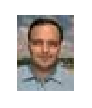
\includegraphics{./figuras/eu.eps}).

O formato em que você deve salvar os arquivos das figuras para que
possa incluí-las no texto depende de como você pretende compilar
o código fonte:
\begin{itemize}
\item se o texto vai ser compilado com \texttt{latex}, todos os
arquivos devem estar no formato EPS (\emph{Encapsulated PostScipt});
\item se o texto vai ser compilado com \texttt{pdflatex}, os
arquivos devem estar nos formatos PDF ou JPEG (outros formatos são
aceitos, mas estes são os recomendáveis).
\end{itemize}
É aconselhável que você não inclua a terminação no nome do arquivo que
é parâmetro para o comando \texttt{includegraphics}. Isto porque, de
acordo com a forma como o texto está sendo compilado, o \LaTeX\
acrescenta a terminação adequada. Por exemplo, caso seu texto inclua o
comando \verb|\includegraphics{eu}|, o \LaTeX\ procurará o arquivo
\texttt{eu.eps} caso esteja sendo chamado via \texttt{latex} ou um dos
arquivos \texttt{eu.pdf} ou \texttt{eu.jpg} caso esteja sendo chamado
via \texttt{pdflatex}.

As figuras podem ser divididas em dois grandes grupos:
\begin{itemize}
\item As imagens e fotos, que normalmente correspondem a visões reais
do mundo e são obtidas por câmeras digitais ou
assemelhados. Caracterizam-se por conterem grandes quantidades de
nuances, texturas e cores.
\item As figuras sintéticas, normalmente produzidas utilizando
\emph{softwares} dedicados. Geralmente contêm figuras geométricas
(linhas, quadrados, etc.), textos e poucas cores e texturas. Neste
grupo, para efeito de discussão das ferramentas de produção, podem-se
identificar duas categorias:
\begin{itemize}
\item Os desenhos e esquemas: diagramas de blocos, organogramas e
fluxogramas, representações esquemáticas, etc.
\item Os gráficos: representações gráficas de valores ou funções
matemáticas.
\end{itemize}
\end{itemize}

\subsection{Imagens e fotos}
\label{Sec:imagens}

As imagens e fotos normalmente só podem ser armazenadas em formatos
que representam cada \emph{pixel} da imagem separadamente,
eventualmente com algum tipo de compressão. Os formatos JPEG, GIF,
TIF, PNM (PBM, PGM ou PPM), BMP (Bitmap) e PNG, entre outros, são
todos desta categoria.  Se sua figura está em algum destes formatos,
você deve convertê-la para EPS (se usar \texttt{latex}) ou para JPEG
(se usar \texttt{pdflatex}) para poder incluí-la no documento \LaTeX.

A quase totalidade dos \emph{softwares} de visualização de imagens
permite salvá-las em múltiplos formatos, geralmente incluindo JPEG e
EPS. No Unix, você dispõe ainda de vários programas para fazer a
conversão em comandos de linha: \texttt{jpegtopnm},
\texttt{pnmtojpeg}, \texttt{pnmtops}, \texttt{gif2ps},
\texttt{giftopnm}, \texttt{tiff2ps}, \texttt{tifftopnm},
\texttt{bmptopnm} e \texttt{pngtopnm}, entre outros.

A figura \ref{Fig:belmonte} mostra um exemplo de inclusão de uma
imagem no texto \LaTeX.

\begin{figure}[htbp!] \begin{center}
% fbox faz uma borda ao redor do seu argumento
\fbox{\includegraphics[width=0.75\linewidth]{./figuras/belmonte}}
\caption{Exemplo de imagem real}
\label{Fig:belmonte}
\end{center} \end{figure}

\subsection{Figuras sintéticas}
\label{Sec:figsinteticas}

As figuras sintéticas podem ser armazenadas em formato
\emph{pixel}-a-\emph{pixel}, como se fossem uma imagem, ou em
formato vetorial. No formato vetorial as primitivas que formam a
figura (linhas, textos, etc.) são descritas pelos parâmetros que as
caracterizam (ponto de início e fim, \emph{string} e posição do texto,
etc.). As figuras em formato vetorial são mais adequadas pois
usualmente correspondem a arquivos menores e a qualidade da imagem
não sofre perdas ao se aumentar ou diminuir o tamanho da figura.

Para inclusão no \LaTeX, os formatos PDF e EPS são os únicos que podem
representar figuras no formato vetorial. Nem toda figura salva nestes
formatos, entretanto, é necessariamente vetorial, pois tanto o PDF
quanto o EPS podem representar tanto figuras em formato
\emph{pixel}-a-\emph{pixel} quanto figuras em formato vetorial. Para
que sua figura seja vetorial, é necessário que o \emph{software} que a
gerou tenha a capacidade de produzi-las.

Para demonstrar a melhor qualidade das figuras em formato vetorial,
nas figuras \ref{Fig:bigvetorial} e \ref{Fig:bigbitmap} se mostra em
tamanho natural um mesmo diagrama nos formatos vetorial e de
\emph{pixels}. Nas figuras \ref{Fig:bigvetorialreduzida} e
\ref{Fig:bigbitmapreduzida} estas mesmas figuras são apresentadas
com uma redução de 50\%, utilizando o parâmetro \texttt{scale} do
\texttt{includegraphics}. Já nas figuras \ref{Fig:smallvetorial} e
\ref{Fig:smallbitmap} o diagrama original foi reduzido, de forma que
seu tamanho natural é menor. Nas figuras
\ref{Fig:smallvetorialampliada} e \ref{Fig:smallbitmapampliada}
este diagrama pequeno está aumentado de um fator arbitrário, calculado
pelo \texttt{includegraphics} para que a imagem ocupe toda a largura
da linha.

\begin{figure}[htbp!] \begin{center}
\includegraphics{./figuras/bigvetorial}
\caption{Figura vetorial grande em tamanho natural}
\vspace{6mm}
\label{Fig:bigvetorial}
\includegraphics{./figuras/bigbitmap}
\caption{Figura \emph{pixel}-a-\emph{pixel} grande em tamanho natural}
\label{Fig:bigbitmap}
\vspace{6mm}
\includegraphics[scale=0.5]{./figuras/bigvetorial}
\caption{Figura vetorial grande em tamanho reduzido}
\label{Fig:bigvetorialreduzida}
\vspace{6mm}
\includegraphics[scale=0.5]{./figuras/bigbitmap}
\caption{Figura \emph{pixel}-a-\emph{pixel} grande em tamanho reduzido}
\label{Fig:bigbitmapreduzida}
\end{center} \end{figure}

\begin{figure}[htbp!] \begin{center}
\includegraphics{./figuras/smallvetorial}
\caption{Figura vetorial pequena em tamanho natural}
\label{Fig:smallvetorial}
\vspace{6mm}
\includegraphics{./figuras/smallbitmap}
\caption{Figura \emph{pixel}-a-\emph{pixel} pequena em tamanho natural}
\label{Fig:smallbitmap}
\vspace{6mm}
\includegraphics[width=\linewidth]{./figuras/smallvetorial}
\caption{Figura vetorial pequena em tamanho ampliado}
\label{Fig:smallvetorialampliada}
\vspace{6mm}
\includegraphics[width=\linewidth]{./figuras/smallbitmap}
\caption{Figura \emph{pixel}-a-\emph{pixel} pequena em tamanho ampliado}
\label{Fig:smallbitmapampliada}
\end{center} \end{figure}

Nota-se que no formato vetorial as
linhas mantêm a espessura mesmo quando se fazem
ampliações ou reduções. Já no formato de \emph{pixels}
as linhas ficam mais claras (cinzas, ao invés de pretas) após as
reduções e mais grossas após as ampliações, além de uma perda geral
de definição da imagem.

\section{Ferramentas para desenhos e esquemas}
\label{Sec:desenhos}

Existem diversas ferramentas para fazer desenhos, mas muitas delas
apenas salvam a figura gerada em formatos \emph{pixel}-a-\emph{pixel}.
No Unix, pode-se utilizar o \texttt{xfig}, que exporta imagens em
muitos formatos, inclusive nos vetoriais (PDF e EPS). Os diagramas das
figuras \ref{Fig:bigvetorial} a \ref{Fig:smallbitmapampliada} foram
desenhados e exportados no \texttt{xfig}. O arquivo fonte
correspondente é o \texttt{diagrama.fig}, no diretório
\texttt{figuras}.

A possibilidade de salvar figuras em modo vetorial impõe que alguns
recursos para desenho de imagens não sejam oferecidos. Um deles é o
desenho a mão-livre, já que seria impossível descrever a curva obtida
em termos de figuras geométricas básicas. Outro recurso inexistente é
o de preencher uma região com uma determinada cor. Esta última
limitação muitas vezes pode ser contornada utilizando-se a noção de
profundidade.  Por exemplo, para desenhar uma figura vazado e
preenchido de azul, pode-se desenhar a figura externa preenchido de
azul sobre o qual se desenha a figura interna preenchido de branco,
como mostram os exemplos da figura~\ref{Fig:circulo}.

\begin{figure}[htb] \begin{center}
\includegraphics{./figuras/circulo}
\caption{Preenchimento de figuras utilizando diferentes profundidades}
\label{Fig:circulo}
\end{center} \end{figure}

A noção de profundidade no \texttt{xfig} foi exaustivamente utilizada
para desenhar os símbolos da UFRN e do PPgEEC que podem ser vistos na
página de rosto deste documento. Os arquivos \texttt{xfig}
correspondentes são \texttt{UFRN.fig} e \texttt{PPgEE.fig}. Ela também
pode ser utilizada para mesclar imagens com figuras sintéticas, como
na figura \ref{Fig:pensador} (veja arquivo \texttt{figuras/pensador.fig}).

\begin{figure}[htb] \begin{center}
\includegraphics{./figuras/pensador}
\caption{Imagem mesclada com elementos sintéticos}
\label{Fig:pensador}
\end{center} \end{figure}

Outra possibilidade oferecida pelo \texttt{xfig} é a inclusão de comandos
\LaTeX\ dentro da figura. Para utilizar este recurso,
marque no \texttt{xfig} os textos que devem ser interpretados como
comandos \LaTeX\ com o \emph{flag} \texttt{special} e exporte a figura
no modo \emph{Combinado PS/Latex} ou \emph{Combinado PDF/Latex}. Veja
um exemplo na figura \ref{Fig:combinado}; note que o arquivo é incluído com
\verb|\input{}| e não com \verb|\includegraphics{}|.

% Note que foi redefinido um comando aqui no texto para ser incluído
% na figura. Isto é para evitar digitação de expressões LaTeX muito
% grandes dentro do xfig
\newcommand{\formulagrande}{$\frac{G_3G_4}{1-G_3G_4H_1}$}
\begin{figure}[htb] \begin{center}
%\input{textuais/04-problema/figuras/combinado.pstex_t} % Se usar latex
\caption{Figura incluindo comandos \LaTeX}
\label{Fig:combinado}
\end{center} \end{figure}

\section{Ferramentas para gráficos}
\label{Sec:graficos}

Gráficos devem ser gerados com aplicativos capazes de exportar o
resultado nos formatos EPS ou PDF, preferencialmente em formato
vetorial. Os conhecidos programas \emph{Scilab} e \emph{Matlab} têm
esta capacidade. Se você deseja algo mais simples, a ferramenta
\textit{GNUplot} é uma das mais utilizadas no Unix para a geração de
gráficos de funções matemáticas.

Uma vez gerados, gráficos são inseridos no texto tal como figuras. A
figura~\ref{fig:grafico} apresenta um gráfico gerado através do
comando de linha \texttt{gnuplot grafico.gnuplot}. Este arquivo
\texttt{grafico.gnuplot}, que contém uma série de comandos do
\textit{GNUplot}, está no diretório \texttt{figuras}.

\begin{figure}[htbp]
\centering
\includegraphics{./figuras/grafico}
\caption{Exemplo de gráfico de funções matemáticas}
\label{fig:grafico}
\end{figure}

\section{Conclusões}

Ferramentas de desenho capazes de gerar a saída em formato vetorial
são mais difíceis de usar e parecem ser dotadas de menos recursos do
que outras que só exportam seus resultados como imagens de
\emph{pixels}.  Isto se deve à necessidade de descrever todos os
elementos da imagem sob a forma de primitivas parametrizáveis para
permitir que elas sejam escaláveis à vontade e exportáveis para
qualquer formato desejado.

Entretanto, a qualidade visual das figuras obtidas e a sua
reusabilidade é muito maior. A comparação é aproximadamente a mesma
que a entre textos produzidos em \LaTeX\ e em editores gráficos. Desta
forma, na medida do possível, tente conjugar a escrita do documento
\LaTeX\ com a utilização de alguma ferramenta de desenho vetorial.

% LocalWords:  editadas PS


% Cap. 5 - Memorial de atuação / CInO
\include{textuais/memoria_atuacao}

% Cap. 6 - Considerações finais
%%
%% Capítulo 4: Figuras, gráficos e tabelas
%%

\mychapter{Experimentos e Resultados}
\label{Cap:ExperimentosResultados}

Esta é a parte mais importante (e interessante) do trabalho. Especifique o ferramental usado para a experimentação empírica da solução implementada. Descreva cada experimento realizado de forma bem explicativa (ou seja, planeje os experimentos). Veja o que experimentar, o que são resultados (erros e métricas usadas para medi-los, medidas estatísticas). Use .e abuse de gráficos, tabelas e figuras mostrando resultados visuais (impressiona). Uma dica interessante: faça um video e coloque no youtube, demonstrando o sistema funcionando (impressiona), citando a URL entre parênteses. Não apenas descreva os experimentos, mas também discuta os resultados e os compare (principalmente) com outros encontrados na literatura (e citados nos trabalhos relacionados).

%Uma das maiores dificuldades na edição de textos de qualidade é o
%posicionamento dos elementos gráficos: figuras, gráficos e
%tabelas. Como estes elementos muitas vezes são grandes, aparece o
%dilema sobre o que fazer quando uma quebra de página deveria acontecer
%no meio do elemento. Há duas possibilidades:
%\begin{enumerate}
%\item O autor informa exatamente onde o elemento gráfico deve ficar no
%texto, evitando que quebras de páginas aconteçam no meio de um
%elemento. O problema com esta abordagem é que todo o trabalho de
%posicionamento pode ser perdido caso se inclua ou se exclua algum
%texto ou elemento.
%\item O editor de texto posiciona os elementos gráficos de forma a não
%deixar espaços em branco nas páginas. Estes elementos que podem ser
%posicionados pelo editor são conhecidos como \emph{elementos
%flutuantes}. O problema com esta abordagem é que o posicionamento
%adotado pode não corresponder às expectativas do autor.
%\end{enumerate}
%
%O \LaTeX\ oferece as duas possibilidades de posicionamento. Este
%capítulo apresenta exemplos de inclusão de elementos gráficos no
%texto, bem como algumas ferramentas externas ao \LaTeX\ que podem ser
%utilizadas para gerá-los.
%
%\section{Elementos flutuantes}
%\label{Sec:flutuantes}
%
%Para caracterizar uma parte do texto como sendo flutuante, ela deve ser
%delimitada por \verb|\begin{figure}| e \verb|\end{figure}| ou por
%\verb|\begin{table}| e \verb|\end{table}|. Apesar do que os nomes
%sugerem, nada obriga que o ambiente \texttt{figure} seja usado para
%delimitar figuras ou que o ambiente \texttt{table} seja usado para
%delimitar tabelas, embora esta seja a escolha quase sempre
%adotada. Estes dois ambientes são praticamente equivalentes, com as
%seguintes diferenças:
%\begin{itemize}
%\item os dois ambientes usam contadores diferentes para numerar os
%elementos flutuantes;
%\item os ambientes \texttt{figure} serão incluídos na
%\texttt{listoffigures}, enquanto os ambientes \texttt{table} serão
%incluídos na \texttt{listoftables};
%\item as legendas (\texttt{caption}'s) dos ambientes \texttt{figure}
%serão precedidas da palavra ``Figura \dots'', enquanto as legendas dos
%ambientes \texttt{table} serão precedidas da palavra ``Tabela \dots''.
%Estas duas palavras podem ser alteradas pelo autor.
%\end{itemize}
%Para ilustrar o fato de que estes ambientes podem conter virtualmente
%qualquer coisa, a figura~\ref{Fig:textoflutuante} contém um texto que
%foi tornado flutuante por ser incluído em um ambiente \texttt{figure}
%e as tabelas \ref{Tab:equacaoflutuante} e \ref{Tab:equacaoflutuante2}
%contêm expressões matemáticas flutuantes, incluídas em um ambiente
%\texttt{table}. A tabela (\texttt{table}) \ref{Tab:submultilinhas} na
%página \pageref{Tab:submultilinhas} também não contém uma tabela no
%sentido estrito do termo, mas sim uma linha de texto formada por duas
%\texttt{minipage}'s separadas por um espaço horizontal. A primeira
%\texttt{minipage} contém um trecho de código fonte e a segunda, o
%resultado produzido (uma expressão matemática multialinhada).
%
%\begin{figure}[tbp]
%\caption{Trecho de \emph{Os Lusíadas}, de Luis de Camões}
%\label{Fig:textoflutuante}
%% hrule - linha horizontal
%\hrule
%% As minipage's são muito úteis para se colocar duas coisas na mesma linha
%\begin{minipage}{0.45\linewidth}
%% flushleft - alinha à esquerda
%\begin{flushleft}
%As armas e os barões assinalados\\
%Que da ocidental praia lusitana\\
%Por mares nunca dantes navegados\\
%Passaram ainda além da Trapobana\\
%Em perigos e guerras esforçados\\
%Mais do que prometia a força humana\\
%Entre gente remota edificaram\\
%Novo reino, que tanto sublimaram
%\end{flushleft}
%\end{minipage}
%\hfill
%\begin{minipage}{0.45\linewidth}
%% flushright - alinha à direita
%\begin{flushright}
%E também as memórias gloriosas\\
%Daqueles reis que foram dilatando\\
%A Fé, o Império, as terras viciosas\\
%De África e Ásia andaram devastando,\\
%E aqueles que por obras valerosas\\
%Se vão da lei da morte libertando:\\
%Cantando espalharei por toda parte,\\
%Se a tanto me ajudar o engenho e arte.
%\end{flushright}
%\end{minipage}
%\hrule
%\end{figure}
%
%\begin{table}[bp]
%% As minipage's são muito úteis para se colocar duas coisas na mesma linha
%\begin{minipage}[b]{0.45\linewidth}
%\begin{center}
%\[
%ax^2 + bx + c = 0
%\]
%\end{center}
%\caption{Equação de segundo grau}
%\label{Tab:equacaoflutuante}
%\end{minipage}
%\hfill
%\begin{minipage}[b]{0.50\linewidth}
%\begin{center}
%\[
%x = \frac{-b\pm\sqrt{b^2-4ac}}{2a}
%\]
%\end{center}
%\caption{Raízes da equação da tabela~\ref{Tab:equacaoflutuante}}
%\label{Tab:equacaoflutuante2}
%\end{minipage}
%\end{table}
%
%É importante ressaltar que o que é numerado é o \texttt{caption} e não
%a \texttt{figure} ou a \texttt{table}. Portanto, o \texttt{label} deve
%ser colocado sempre após o \texttt{caption} ao qual ele se
%refere. Conforme ilustram as tabelas \ref{Tab:equacaoflutuante} e
%\ref{Tab:equacaoflutuante2}, uma mesma \texttt{figure} ou
%\texttt{table} pode ter mais de um ou nenhum \texttt{caption}.
%O \texttt{caption} pode ser colocado antes do conteúdo flutuante, como
%na figura \ref{Fig:textoflutuante}, ou depois, como nas tabelas
%\ref{Tab:equacaoflutuante} e \ref{Tab:equacaoflutuante2}. Nos
%documentos do PPgEE, o padrão é sempre posicionar o \texttt{caption}
%abaixo das figuras e das tabelas.
%
%\subsection{Posicionamento dos elementos flutuantes}
%\label{Sec:posicionamento}
%
%Em cada \verb|\begin{figure}| ou \verb|\begin{table}| pode-se incluir
%um parâmetro opcional com as opções de posicionamento para este
%elemento flutuante. Parâmetros adicionais de comandos \LaTeX\ são
%sempre fornecidos entre colchetes \texttt{[]}, enquanto os parâmetros
%obrigatórios aparecem entre chaves \verb|{}|. As opções disponíveis
%incluem as seguintes:
%\begin{itemize}
%\item[\tt h] O elemento pode ser posicionado na mesma posição em que ele
%aparece no código fonte do texto.
%\item[\tt t] O elemento pode ser posicionado no topo de uma página.
%\item[\tt b] O elemento pode ser posicionado no fim de uma página.
%\item[\tt p] O elemento pode ser incluído em uma página formada só por
%flutuantes.
%\item[\tt !] Normalmente o \LaTeX\ faz algumas considerações de ordem
%estética no posicionamento dos flutuantes, o que às vezes faz com que
%alguns elementos sejam posicionados muito longe de onde são citados,
%principalmente se você não incluir a opção \texttt{p}. Para fazer com
%que as considerações estéticas não sejam levadas em conta para um dado
%elemento, inclua a opção \texttt{!}.
%\end{itemize}
%
%\section{Tabelas em \LaTeX}
%\label{Sec:tabelas}
%
%Tabelas são construídas com comandos próprios do \LaTeX, notadamente o
%ambiente \texttt{tabular}. Nada obriga a que o ambiente
%\texttt{tabular} esteja sempre posicionado em um elemento
%flutuante. Se você quiser impor que uma tabela fique obrigatoriamente
%em uma determinada posição do texto, basta não colocar o
%\texttt{tabular} dentro de um \texttt{table}. Tabelas podem até ser
%incluídas no meio de uma frase.  Por exemplo, eu posso dizer que se um
%jogo da velha está na configuração \textsf{\tiny\begin{tabular}{c|c|c}
%x & & x \\ \hline & & o \\ \hline x & o & \end{tabular}} e se o
%jogador ``\textsf{x}'' sabe jogar, então o jogador ``\textsf{o}'' irá
%perder, independentemente da jogada que faça.
%
%O ambiente \texttt{tabular} tem um parâmetro obrigatório que indica o
%número de colunas da tabela e o posicionamento dos objetos em cada
%coluna. Por exemplo, uma tabela criada com \verb|\begin{tabular}{lcr}|
%terá três colunas; o texto será alinhado à esquerda na primeira
%coluna, centralizado na segunda e alinhado à direita na
%terceira. Podem ser incluídos objetos que ocupam mais de uma linha
%(comando \texttt{multirow}) ou mais de uma coluna (comando
%\texttt{multicolumn}). Neste último caso, também é possível mudar o
%alinhamento do texto. Exemplos podem ser vistos nas tabelas
%\ref{Tab:multilinhas} e \ref{Tab:submultilinhas}, na
%página~\pageref{Tab:multilinhas}.
%
%Com o pacote \texttt{tabularx}, além das opções normais de
%posicionamento de colunas (\texttt{lcr}), pode-se incluir
%automaticamente um texto qualquer antes de cada elemento da coluna
%(\verb|>{}|). Este recurso foi utilizado nas tabelas
%\ref{Tab:multilinhas} e \ref{Tab:submultilinhas} para fazer
%com que todos os textos de algumas colunas fossem automaticamente
%escritos na fonte \texttt{tt}. Além disso, podem-se criar colunas de
%largura fixa e/ou de largura que se ajustam para que a tabela ocupe
%toda a largura desejada, além do estilo tradicional de coluna que
%assume a largura suficiente para conter seus elementos. Exemplos de
%colunas com diferentes larguras e alinhamentos podem ser vistos na
%tabela \ref{Tab:larguracolunas}.
%
%\begin{table}[htbp]
%\begin{tabularx}{\linewidth}{|p{3cm}|X|l|} \hline
%COLUNA p & COLUNA X & COLUNA l \\ \hline
%Largura fixa (não depende do conteúdo) &
%Expandível &
%Ajustável \\ \hline
%Alinhada no topo &
%Alinhada à esquerda &
%Alinhada à esquerda \\ \hline
%\end{tabularx}
%\\[0.5cm]
%\begin{tabularx}{\linewidth}{|b{3cm}|C|r|} \hline
%COLUNA b & COLUNA C (ver \texttt{comandos.tex}) & COLUNA r \\ \hline
%Largura fixa (não depende do conteúdo) &
%Expandível &
%Ajustável \\ \hline
%Alinhada na base &
%Centralizada &
%Alinhada à direita \\ \hline
%\end{tabularx}
%\caption{Tabelas com colunas de diferentes larguras e alinhamentos}
%\label{Tab:larguracolunas}
%\end{table}
%
%\section{Figuras em \LaTeX}
%\label{Sec:figuras}
%
%As figuras (imagens, desenhos, gráficos, etc.) devem ser produzidas
%por ferramentas externas ao \LaTeX, salvas em um arquivo e inseridas
%no texto usando o comando \texttt{includegraphics}. Da mesma forma
%que as tabelas, as figuras podem ser flutuantes, caso sejam
%inseridas dentro de um ambiente \texttt{figure}, ou ter uma posição
%fixa no texto (como aqui: \includegraphics{textuais/04-figuras/figuras/eu}).
%
%O formato em que você deve salvar os arquivos das figuras para que
%possa incluí-las no texto depende de como você pretende compilar
%o código fonte:
%\begin{itemize}
%\item se o texto vai ser compilado com \texttt{latex}, todos os
%arquivos devem estar no formato EPS (\emph{Encapsulated PostScipt});
%\item se o texto vai ser compilado com \texttt{pdflatex}, os
%arquivos devem estar nos formatos PDF ou JPEG (outros formatos são
%aceitos, mas estes são os recomendáveis).
%\end{itemize}
%É aconselhável que você não inclua a terminação no nome do arquivo que
%é parâmetro para o comando \texttt{includegraphics}. Isto porque, de
%acordo com a forma como o texto está sendo compilado, o \LaTeX\
%acrescenta a terminação adequada. Por exemplo, caso seu texto inclua o
%comando \verb|\includegraphics{eu}|, o \LaTeX\ procurará o arquivo
%\texttt{eu.eps} caso esteja sendo chamado via \texttt{latex} ou um dos
%arquivos \texttt{eu.pdf} ou \texttt{eu.jpg} caso esteja sendo chamado
%via \texttt{pdflatex}.
%
%As figuras podem ser divididas em dois grandes grupos:
%\begin{itemize}
%\item As imagens e fotos, que normalmente correspondem a visões reais
%do mundo e são obtidas por câmeras digitais ou
%assemelhados. Caracterizam-se por conterem grandes quantidades de
%nuances, texturas e cores.
%\item As figuras sintéticas, normalmente produzidas utilizando
%\emph{softwares} dedicados. Geralmente contêm figuras geométricas
%(linhas, quadrados, etc.), textos e poucas cores e texturas. Neste
%grupo, para efeito de discussão das ferramentas de produção, podem-se
%identificar duas categorias:
%\begin{itemize}
%\item Os desenhos e esquemas: diagramas de blocos, organogramas e
%fluxogramas, representações esquemáticas, etc.
%\item Os gráficos: representações gráficas de valores ou funções
%matemáticas.
%\end{itemize}
%\end{itemize}
%
%\subsection{Imagens e fotos}
%\label{Sec:imagens}
%
%As imagens e fotos normalmente só podem ser armazenadas em formatos
%que representam cada \emph{pixel} da imagem separadamente,
%eventualmente com algum tipo de compressão. Os formatos JPEG, GIF,
%TIF, PNM (PBM, PGM ou PPM), BMP (Bitmap) e PNG, entre outros, são
%todos desta categoria.  Se sua figura está em algum destes formatos,
%você deve convertê-la para EPS (se usar \texttt{latex}) ou para JPEG
%(se usar \texttt{pdflatex}) para poder incluí-la no documento \LaTeX.
%
%A quase totalidade dos \emph{softwares} de visualização de imagens
%permite salvá-las em múltiplos formatos, geralmente incluindo JPEG e
%EPS. No Unix, você dispõe ainda de vários programas para fazer a
%conversão em comandos de linha: \texttt{jpegtopnm},
%\texttt{pnmtojpeg}, \texttt{pnmtops}, \texttt{gif2ps},
%\texttt{giftopnm}, \texttt{tiff2ps}, \texttt{tifftopnm},
%\texttt{bmptopnm} e \texttt{pngtopnm}, entre outros.
%
%A figura \ref{Fig:belmonte} mostra um exemplo de inclusão de uma
%imagem no texto \LaTeX.
%
%\begin{figure}[htbp!] \begin{center}
%% fbox faz uma borda ao redor do seu argumento
%\fbox{\includegraphics[width=0.75\linewidth]{textuais/04-figuras/figuras/belmonte}}
%\caption{Exemplo de imagem real}
%\label{Fig:belmonte}
%\end{center} \end{figure}
%
%\subsection{Figuras sintéticas}
%\label{Sec:figsinteticas}
%
%As figuras sintéticas podem ser armazenadas em formato
%\emph{pixel}-a-\emph{pixel}, como se fossem uma imagem, ou em
%formato vetorial. No formato vetorial as primitivas que formam a
%figura (linhas, textos, etc.) são descritas pelos parâmetros que as
%caracterizam (ponto de início e fim, \emph{string} e posição do texto,
%etc.). As figuras em formato vetorial são mais adequadas pois
%usualmente correspondem a arquivos menores e a qualidade da imagem
%não sofre perdas ao se aumentar ou diminuir o tamanho da figura.
%
%Para inclusão no \LaTeX, os formatos PDF e EPS são os únicos que podem
%representar figuras no formato vetorial. Nem toda figura salva nestes
%formatos, entretanto, é necessariamente vetorial, pois tanto o PDF
%quanto o EPS podem representar tanto figuras em formato
%\emph{pixel}-a-\emph{pixel} quanto figuras em formato vetorial. Para
%que sua figura seja vetorial, é necessário que o \emph{software} que a
%gerou tenha a capacidade de produzi-las.
%
%Para demonstrar a melhor qualidade das figuras em formato vetorial,
%nas figuras \ref{Fig:bigvetorial} e \ref{Fig:bigbitmap} se mostra em
%tamanho natural um mesmo diagrama nos formatos vetorial e de
%\emph{pixels}. Nas figuras \ref{Fig:bigvetorialreduzida} e
%\ref{Fig:bigbitmapreduzida} estas mesmas figuras são apresentadas
%com uma redução de 50\%, utilizando o parâmetro \texttt{scale} do
%\texttt{includegraphics}. Já nas figuras \ref{Fig:smallvetorial} e
%\ref{Fig:smallbitmap} o diagrama original foi reduzido, de forma que
%seu tamanho natural é menor. Nas figuras
%\ref{Fig:smallvetorialampliada} e \ref{Fig:smallbitmapampliada}
%este diagrama pequeno está aumentado de um fator arbitrário, calculado
%pelo \texttt{includegraphics} para que a imagem ocupe toda a largura
%da linha.
%
%\begin{figure}[htbp!] \begin{center}
%\includegraphics{textuais/04-figuras/figuras/bigvetorial}
%\caption{Figura vetorial grande em tamanho natural}
%\vspace{6mm}
%\label{Fig:bigvetorial}
%\includegraphics{textuais/04-figuras/figuras/bigbitmap}
%\caption{Figura \emph{pixel}-a-\emph{pixel} grande em tamanho natural}
%\label{Fig:bigbitmap}
%\vspace{6mm}
%\includegraphics[scale=0.5]{textuais/04-figuras/figuras/bigvetorial}
%\caption{Figura vetorial grande em tamanho reduzido}
%\label{Fig:bigvetorialreduzida}
%\vspace{6mm}
%\includegraphics[scale=0.5]{textuais/04-figuras/figuras/bigbitmap}
%\caption{Figura \emph{pixel}-a-\emph{pixel} grande em tamanho reduzido}
%\label{Fig:bigbitmapreduzida}
%\end{center} \end{figure}
%
%\begin{figure}[htbp!] \begin{center}
%\includegraphics{textuais/04-figuras/figuras/smallvetorial}
%\caption{Figura vetorial pequena em tamanho natural}
%\label{Fig:smallvetorial}
%\vspace{6mm}
%\includegraphics{textuais/04-figuras/figuras/smallbitmap}
%\caption{Figura \emph{pixel}-a-\emph{pixel} pequena em tamanho natural}
%\label{Fig:smallbitmap}
%\vspace{6mm}
%\includegraphics[width=\linewidth]{textuais/04-figuras/figuras/smallvetorial}
%\caption{Figura vetorial pequena em tamanho ampliado}
%\label{Fig:smallvetorialampliada}
%\vspace{6mm}
%\includegraphics[width=\linewidth]{textuais/04-figuras/figuras/smallbitmap}
%\caption{Figura \emph{pixel}-a-\emph{pixel} pequena em tamanho ampliado}
%\label{Fig:smallbitmapampliada}
%\end{center} \end{figure}
%
%Nota-se que no formato vetorial as
%linhas mantêm a espessura mesmo quando se fazem
%ampliações ou reduções. Já no formato de \emph{pixels}
%as linhas ficam mais claras (cinzas, ao invés de pretas) após as
%reduções e mais grossas após as ampliações, além de uma perda geral
%de definição da imagem.
%
%\section{Ferramentas para desenhos e esquemas}
%\label{Sec:desenhos}
%
%Existem diversas ferramentas para fazer desenhos, mas muitas delas
%apenas salvam a figura gerada em formatos \emph{pixel}-a-\emph{pixel}.
%No Unix, pode-se utilizar o \texttt{xfig}, que exporta imagens em
%muitos formatos, inclusive nos vetoriais (PDF e EPS). Os diagramas das
%figuras \ref{Fig:bigvetorial} a \ref{Fig:smallbitmapampliada} foram
%desenhados e exportados no \texttt{xfig}. O arquivo fonte
%correspondente é o \texttt{diagrama.fig}, no diretório
%\texttt{figuras}.
%
%A possibilidade de salvar figuras em modo vetorial impõe que alguns
%recursos para desenho de imagens não sejam oferecidos. Um deles é o
%desenho a mão-livre, já que seria impossível descrever a curva obtida
%em termos de figuras geométricas básicas. Outro recurso inexistente é
%o de preencher uma região com uma determinada cor. Esta última
%limitação muitas vezes pode ser contornada utilizando-se a noção de
%profundidade.  Por exemplo, para desenhar uma figura vazado e
%preenchido de azul, pode-se desenhar a figura externa preenchido de
%azul sobre o qual se desenha a figura interna preenchido de branco,
%como mostram os exemplos da figura~\ref{Fig:circulo}.
%
%\begin{figure}[htb] \begin{center}
%\includegraphics{textuais/04-figuras/figuras/circulo}
%\caption{Preenchimento de figuras utilizando diferentes profundidades}
%\label{Fig:circulo}
%\end{center} \end{figure}
%
%A noção de profundidade no \texttt{xfig} foi exaustivamente utilizada
%para desenhar os símbolos da UFRN e do PPgEE que podem ser vistos na
%página de rosto deste documento. Os arquivos \texttt{xfig}
%correspondentes são \texttt{UFRN.fig} e \texttt{PPgEE.fig}. Ela também
%pode ser utilizada para mesclar imagens com figuras sintéticas, como
%na figura \ref{Fig:pensador} (veja arquivo \texttt{figuras/pensador.fig}).
%
%\begin{figure}[htb] \begin{center}
%\includegraphics{textuais/04-figuras/figuras/pensador}
%\caption{Imagem mesclada com elementos sintéticos}
%\label{Fig:pensador}
%\end{center} \end{figure}
%
%Outra possibilidade oferecida pelo \texttt{xfig} é a inclusão de comandos
%\LaTeX\ dentro da figura. Para utilizar este recurso,
%marque no \texttt{xfig} os textos que devem ser interpretados como
%comandos \LaTeX\ com o \emph{flag} \texttt{special} e exporte a figura
%no modo \emph{Combinado PS/Latex} ou \emph{Combinado PDF/Latex}. Veja
%um exemplo na figura \ref{Fig:combinado}; note que o arquivo é incluído com
%\verb|\input{}| e não com \verb|\includegraphics{}|.
%
%% Note que foi redefinido um comando aqui no texto para ser incluído
%% na figura. Isto é para evitar digitação de expressões LaTeX muito
%% grandes dentro do xfig
%\newcommand{\formulagrande}{$\frac{G_3G_4}{1-G_3G_4H_1}$}
%\begin{figure}[htb] \begin{center}
%%\input{figuras/combinado.pstex_t} % Se usar latex
%\input{textuais/04-figuras/figuras/combinado.pdftex_t} % Se usar pdflatex
%\caption{Figura incluindo comandos \LaTeX}
%\label{Fig:combinado}
%\end{center} \end{figure}
%
%\section{Ferramentas para gráficos}
%\label{Sec:graficos}
%
%Gráficos devem ser gerados com aplicativos capazes de exportar o
%resultado nos formatos EPS ou PDF, preferencialmente em formato
%vetorial. Os conhecidos programas \emph{Scilab} e \emph{Matlab} têm
%esta capacidade. Se você deseja algo mais simples, a ferramenta
%\textit{GNUplot} é uma das mais utilizadas no Unix para a geração de
%gráficos de funções matemáticas.
%
%Uma vez gerados, gráficos são inseridos no texto tal como figuras. A
%figura~\ref{fig:grafico} apresenta um gráfico gerado através do
%comando de linha \texttt{gnuplot grafico.gnuplot}. Este arquivo
%\texttt{grafico.gnuplot}, que contém uma série de comandos do
%\textit{GNUplot}, está no diretório \texttt{figuras}.
%
%\begin{figure}[htbp]
%\centering
%\includegraphics{textuais/04-figuras/figuras/grafico}
%\caption{Exemplo de gráfico de funções matemáticas}
%\label{fig:grafico}
%\end{figure}
%
%\section{Conclusões}
%
%Ferramentas de desenho capazes de gerar a saída em formato vetorial
%são mais difíceis de usar e parecem ser dotadas de menos recursos do
%que outras que só exportam seus resultados como imagens de
%\emph{pixels}.  Isto se deve à necessidade de descrever todos os
%elementos da imagem sob a forma de primitivas parametrizáveis para
%permitir que elas sejam escaláveis à vontade e exportáveis para
%qualquer formato desejado.
%
%Entretanto, a qualidade visual das figuras obtidas e a sua
%reusabilidade é muito maior. A comparação é aproximadamente a mesma
%que a entre textos produzidos em \LaTeX\ e em editores gráficos. Desta
%forma, na medida do possível, tente conjugar a escrita do documento
%\LaTeX\ com a utilização de alguma ferramenta de desenho vetorial.
%
%% LocalWords:  editadas PS


% Cap. 7 - Conclusão
%%
%% Capítulo 5: Conclusões
%%

\mychapter{Conclusão}
\label{Cap:Conclusao}

O capítulo final depende do tipo de documento. Nas propostas de tema
deve ser apresentado de forma clara e sucinta o assunto a ser
desenvolvido e o cronograma de execução do trabalho. Nas teses e
dissertações devem ser ressaltadas as principais contribuições do
trabalho e as suas limitações.

As contribuições devem evitar as adjetivações e julgamentos de valor.
Quanto às limitações, não tenha medo de as apresentar: é muito mais
reconhecido um autor que apresenta os casos em que sua proposta não se
aplica do que outro que parece não ter consciência deles.

Escreva (com outras palavras) o que foi realizado e como foi realizado, o que o trabalho descrito no artigo conseguiu melhorar e qual a sua relevância, e quais são as vantagens e limitações das propostas que a tese/dissertação apresenta. Apresente também eventuais aplicações dos resultados obtidos (ou da metodologia, técnica, produto) e ideias de trabalhos futuro que possam melhorar o seu (não apenas apresente, mas indique como pode ser feito).

%\section{Encadernação}
%
%As propostas de tema e as versões iniciais das teses e dissertações
%são impressas em lado único da folha e em espaçamento um e meio. Para
%a encadernação, usa-se geralmente um método simples, tal como espiral
%na lateral das folhas e capa plástica transparente. O número de cópias
%é igual ao número de membros da banca e pelo menos mais uma (para o
%aluno).
%
%As versões finais das teses e dissertações são impressas em frente e
%verso e em espaçamento simples. O número mínimo de cópias é o seguinte:
%\begin{itemize}
%\item 3 cópias para o PPgEEC e a UFRN.
%\item 1 cópia para cada examinador externo que participou da banca.
%\item ao menos 1 cópia para o aluno (não obrigatória).
%\item 1 cópia para o orientador (por cortesia, não obrigatória)
%\end{itemize}
%
%Para a encadernação, deve-se adotar uma capa rígida de cor azul para
%as dissertações de mestrado e de cor preta para as teses de doutorado,
%ambas com letras douradas. Na capa deve constar o título do
%trabalho, o autor e o ano da defesa. Se possível, a mesma informação
%deve ser repetida na lombada do livro.
%
%Para as versões finais, também se exige uma cópia eletrônica (formato
%PDF) do texto, bem como outros dados. Maiores informações podem ser
%obtidas na página do PPgEEC: \url{http://www.ppgeec.ufrn.br/}

\section{Etapas de Homologação do Título}

Depois de defendido, o seu trabalho passará por um processo de homologação. Atualmente, este pode ser feito e acompanhado via SiGAA, menu Ensino $\rightarrow$ Produções Acadêmicas $\rightarrow$ Acompanhar Procedimentos após Defesa.
\begin{enumerate}
	\item A consolidação da atividade de defesa;
	\item A submissão da versão final corrigida da dissertação. Nesta etapa, o seu orientador irá verificar se as falhas apontadas pela banca foram corrigidas. Caso isto tenha acontecido, a sua dissertação/tese será considerada aprovada, passando para a próxima etapa. Caso contrário, você terá que submeter uma nova versão final, para corrigir os erros apontados pelo seu orientador;
	\item A submissão da versão final com a ficha catalográfica, cujas informações podem ser obtidas na biblioteca central, ou solicitadas pelo SiGAA, no \textit{link} ``Solicitar Ficha Catalográfica''. Esta também será avaliada pelo seu orientador. Caso seja aprovada, virá o próximo passo;
	\item A assinatura do termo de autorização da publicação, que pode ser feita via SiGAA, menu Ensino $\rightarrow$ Termo de Autorização;
	\item O envio da versão final para a avaliação da coordenação. Neste ponto será avaliado se o sua monografia/tese satisfaz os requisitos estabelecidos pelo programa. Aqui, \textbf{é muito importante que todas as considerações fornecidas neste modelo seja seguidas rigorosamente}, caso contrário, o seu trabalho será reenviado para fazer as correções necessárias. Caso esteja conforme o exigido pela coordenação, este será aprovado;
	\item A solicitação de homologação do diploma, que pode ser ser acompanhada na Pro-Reitoria de Pós-Graduação.
\end{enumerate}

\section{Para saber mais}

Procure no Google, ora! Brincadeiras a parte, existem inúmeros
tutoriais sobre \LaTeX\ na rede que podem dar maiores informações
sobre o aplicativo. Para conhecer os pacotes disponíveis, uma opção é
o livro \emph{The \LaTeX\ Companion} \cite{LATEX04}, popularmente
conhecido como o ``livro do cachorro''. Outras informações sobre
redação técnica e normas para confecção de teses e dissertações podem
ser encontradas em livros de Metodologia Científica.


% Referências bibliogáficas (geradas automaticamente)
% Aqui, o comando \phantomsection é utilizado para auxiliar o pacote "hyperref" a fazer a
% referência correta dos links das referências bibliográficas com a página respectiva.
% Caso seja tirado, o "hyperref" irá apontar o link das referências bibliográficas para a
% última subseção da conclusão.
\phantomsection
\addcontentsline{toc}{chapter}{Referências bibliográficas}
\bibliography{bibliografia/bibliografia}

\appendix

%Apêndice A
%%
%% Capítulo 5: Conclusões
%%

\mychapter{Informações adicionais}
\label{Cap:apendice}

Os apêndices são normalmente empregados para incluir informações
adicionais a serem eventualmente consultadas mas que não são
essenciais para a compreensão do texto.

Evite sobrecarregar seu texto com informações longas e de pouco
interesse para uma primeira leitura. São normalmente colocados
nos apêndices:
\begin{itemize}
\item longas deduções ou demonstrações de fórmulas e teoremas;
\item especificações técnicas de equipamentos e descrições de
experimentos;
\item eventuais conhecimentos disponíveis na literatura mas que
se julga conveniente repetir no texto para facilitar a compreensão
do leitor não familiarizado com a área;
\item outras informações que se julga que devam ser preservadas
mas que não são importantes no documento, tais como diagramas
esquemáticos, algoritmos ou trechos de código-fonte, folhas de
especificações, etc.
\end{itemize}


\end{document}
